\documentclass[12pt,a4paper,polish,thesis]{dcsbook}

\usepackage[utf8]{inputenc}
\usepackage{babel}
\usepackage{graphicx} \graphicspath{ {images/} }
\usepackage[hidelinks]{hyperref}
\usepackage[section]{placeins}
\setcounter{secnumdepth}{4}
\setcounter{tocdepth}{3}

\newcommand*{\captionsource}[2]{%
	\caption[{#1}]{%
		#1%
		\\\hspace{\linewidth}%
		\textbf{Źródło: }\raggedright{#2}%
	}%
}

\linespread{1.3}

%\expandafter\def\expandafter\UrlBreaks\expandafter{\UrlBreaks%  save the current one
%	\do\a\do\b\do\c\do\d\do\e\do\f\do\g\do\h\do\i\do\j%
%	\do\k\do\l\do\m\do\n\do\o\do\p\do\q\do\r\do\s\do\t%
%	\do\u\do\v\do\w\do\x\do\y\do\z\do\A\do\B\do\C\do\D%
%	\do\E\do\F\do\G\do\H\do\I\do\J\do\K\do\L\do\M\do\N%
%	\do\O\do\P\do\Q\do\R\do\S\do\T\do\U\do\V\do\W\do\X%
%	\do\Y\do\Z}

\begin{document}

	\author{Tymoteusz Bleja \and Paweł Husak \and Patryk Imosa \and Magalena Łątkowska}
	\title{Internetowa gra edukacyjna ucząca podstaw pracy~z~programem~git}
	\subtitle{Praca inżynierska}
	\supervisor{dr~hab.~inż.~Marek Andrzej Wojciechowski}
	\date{Poznań, 2017}
	\maketitle
	\frontmatter
	\tableofcontents{}
	\mainmatter

	\chapter{Wstęp}

	\section{Zasady odnośnie pisania pracy}

	\begin{itemize}
		\item Piszemy w formie bezosobowej. Można też niby w 1.os liczby mnogiej czyli "Zrobiliśmy...", ale niektórzy akceptują tylko bezosobową, czyli "Zrobiono...".

		\item słów niepolskich - ,,Nie można więc bezpośrednio
		w tekście używać słów angielskich. Jeżeli już — powinny być wyróżnione kursywą'' - niektórzy podobno bardzo hejcą za angielskie słowa niestety.

		\item Jak chodzi o bibliografię, to w wolnej chwili dołączcie linki do stron z jakich korzystaliście, ja to potem ogarnę i zapiszę w takiej formie jak trzeba. Ale spokojnie, bo robienie bibliografii raczej zostawię na koniec.

		\item Ogólnie nie przejmujcie się strukturą, formatowaniem czy innymi formalnymi bzdetami, ja potem będę to ogarniać żeby było wg zasad więc nie traćcie czasu na ogarnianie takich rzeczy.
	\end{itemize}

	Między innymi:
	skąd wgl pomysł - bo Git jest super i konieczny a ciężko się go samemu nauczyć, nauka z wielu źródeł jest chujowa, większość ma tylko blade pojęcie a potem idzie do pracy i dupa - co z tego że nauczyli się na studiach programować jak nie potrafią korzystać z Gita i współpracować z zespołem

	\section*{Cel i zakres pracy}

	cel - nauka fajna łatwa i przyjemna, oraz praktyczna, obycie z typowymi scenariuszami jakie mogą być potrzebne w pracy

	Coś o tym dlaczego akurat przeglądarkowa gra, czemu z grafiką 3D itp.

	Cytat z karty pracy : Zapoznanie się z systemem Git. Opracowanie koncepcji interaktywnego samouczka do nauki podstaw korzystania z systemu Git.  Opracowanie architektury systemu. Implementacja i testowanie systemu. Przygotowanie dokumentacji technicznej i użytkowej.

	\chapter{Podstawy teoretyczne}

	Systemy kontroli wersji służą do przechowywania historii plików, czyli jak sama nazwa wskazuje do kontrolowania ich różnych wersji. Dzięki temu można sprawdzić, jak zmodyfikowany został plik, a w razie potrzeby przywrócić jego poprzedni stan. Jest to szczególnie przydatne w sytuacji, w której zajdzie konieczność wycofania wprowadzonych zmian, na przykład z powodu zmiany koncepcji lub błędów.

	 W~przypadku współpracy grupy osób nad jednym projektem systemy kontroli wersji pełnią często kluczową rolę. Pomagają łączyć zmiany wprowadzone przez różne osoby na tych samych plikach i~służą jako narzędzie do komunikacji i~synchronizacji zmian. Najczęściej są wykorzystywane przy wytwarzaniu oprogramowania, ale mogą być używane także do kontroli jakichkolwiek plików. Ich zastosowanie zastępuje popularną ze względu na swoją prostotę metodę robienia kopii zapasowych na dysku, polegającą na zwykłym przekopiowywaniu plików.

	Wyróżnia się trzy podstawowe rodzaje systemów kontroli wersji.
	\begin{itemize}
		\item \textbf{Lokalne} --- umożliwiające pracę na jednym komputerze, nie pozwalające na synchronizację ze zdalnym repozytorium. Wykorzystywane są rzadko, głównie w~przypadku samodzielnej pracy nad indywidualnym projektem.
		\item \textbf{Scentralizowane} --- korzystające z~architektury klient-serwer, w~której repozytorium przechowywane jest na jednym zdalnym serwerze, z~którym synchronizują się wszyscy użytkownicy.
		\item \textbf{Rozproszone} --- wykorzystujące model P2P, w~którym wszystkie komputery są sobie równoważne (nie ma jednego określonego serwera), a~kopie repozytorium znajdują się na każdej z~jednostek.
	\end{itemize}

	Porządek, w~jakim zostały wymienione rodzaje systemów, jest nieprzypadkowy, odzwierciedla bowiem w~jakiej kolejności powstawały. Przed rozwinięciem się systemów rozproszonych przeważały systemy scentralizowane. Obecnie do wytwarzania oprogramowania najczęściej wykorzystywane są rozproszone systemy kontroli wersji, zapewniające największy stopień bezpieczeństwa danych. W~przypadku awarii serwera w~scentralizowanym systemie utracone zostaje całe repozytorium. Może zostać odzyskane jedynie z~kopii zapasowych, pod warunkiem, że zostały one wcześniej wykonane. Korzystając z~rozproszonej kontroli wersji odzyskanie repozytorium po awarii jednej jednostki nie stanowi poważnego problemu, ponieważ na każdym komputerze znajduje się jego kopia.

	\begin{figure}[h]
		\centering
		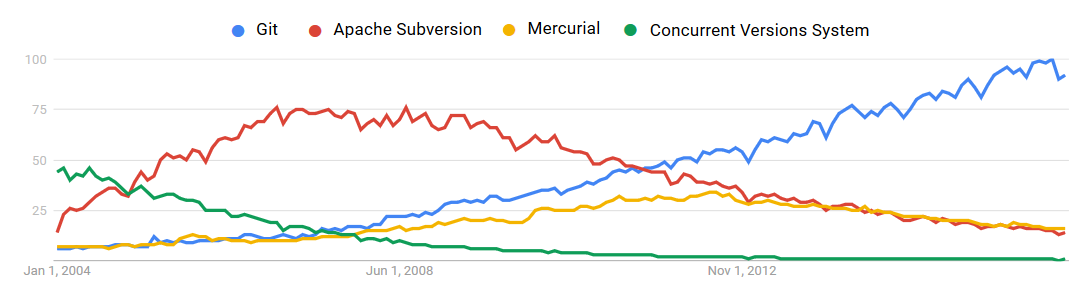
\includegraphics[width=16cm]{vcs_interest}
		\captionsource{Zainteresowanie systemami kontroli wersji w wyszukiwarce Google, dane od stycznia 2004 do stycznia 2017}{\url{https://www.google.com/trends/explore?date=2004-01-01\%202017-01-01\&q=\%2Fm\%2F05vqwg,\%2Fm\%2F012ct9,\%2Fm\%2F08441\_,\%2Fm\%2F09d6g\&hl=en-US}}
		\label{fig:vcs_interest}
	\end{figure}

	Na rysunku~\ref{fig:vcs_interest} przedstawiony jest wykres ilustrujący relatywną popularność czterech znanych systemów kontroli wersji w~wyszukiwarce Google, na przestrzeni ostatnich 13~lat. Uwzględnione zostały dwa scentralizowane (CVS i~Subversion) oraz dwa rozproszone systemy kontroli wersji (Git i~Mercurial). Wyraźnie widać, że popularność tych pierwszych znacząco spadła względem rozproszonego modelu, który wciąż zyskuje na popularności. Przewaga systemu Git nad pozostałymi nie ulega wątpliwości, jest on aktualnie ponad czterokrotnie częściej wyszukiwany w~Google niż Mercurial czy Subversion, co przekłada się na stale rosnącą liczbę użytkowników.

	Obecnie systemy kontroli wersji są tak popularne, że zdecydowana większość programistów korzysta z~nich na~co~dzień. Praca polegająca na wytwarzaniu oprogramowania wykonywana jest najczęściej zespołowo, a~do efektywnej współpracy system kontroli wersji jest bezwzględnie potrzebny. Znajomość i~umiejętność sprawnego korzystania z takich systemów jest więc niezbędna programistom, którzy zamierzają pracować w~większych przedsiębiorstwach i~korporacjach.

	\section{System kontroli wersji Git}

	System kontroli wersji Git stworzony został w 2005 roku, przez zespół programistów pracujących wspólnie nad jądrem Linuksa, w~tym przez Linusa Torvaldsa, twórcę wspomnianego systemu operacyjnego. Wykorzystywali oni wcześniej inny darmowy rozproszony system kontroli wersji, który przestał być ogólnodostępny. W~związku z~tym postanowili napisać własny, doskonalszy od~poprzedniego. Z~założenia miał to~być szybki, rozproszony system, wspierający współbieżną pracę nad różnymi aspektami i~dobrze radzący sobie z~ogromnymi projektami, takimi jak jądro Linuksa.

	\subsection{Cechy charakterystyczne}
	Stworzony przez Linusa Torvaldsa system kontroli wersji Git różni się znacząco od wcześniejszych systemów, szczególnie tych scentralizowanych. W odmienny sposób przechowuje nowe wersje plików. W przeciwieństwie do poprzedników zapamiętuje cały stan repozytorium, a~nie jedynie różnicę pomiędzy plikami. Dla zwiększenia efektywności, jeśli plik nie został zmodyfikowany, to nie jest kopiowany tylko przechowywana jest referencja do~jego aktualnej wersji.

	Kolejną istotną różnicą jest możliwość pracy lokalnej, bez ciągłej potrzeby łączenia się z~serwerem, nawet przy pracy nad projektem zespołowym. System Git pozwala wprowadzać zmiany i~zatwierdzać je bez dostępu do sieci. Komunikacja z innymi jednostkami w~celu synchronizacji danych może odbyć się w~dowolnym momencie. Wcześniejsze scentralizowane systemy, takie jak Subversion, nie pozwalały na taki model pracy. Większość operacji wymagała połączenia z~serwerem, co~wpływało na dłuższy czas wykonywania.

	Git przypisuje do zapisanych stanów projektu czterdziestoznakowe skróty SHA-1. Dzięki tym sumom kontrolnym zauważy każdą, nawet najmniejszą zmianę wprowadzoną na kontrolowanym pliku, niezależnie od sposobu przeprowadzenia modyfikacji.

	Jako najważniejszą zaletę systemu Git powszechnie uznaje się efektywny system rozgałęziania i~łączenia gałęzi. W~przeciwieństwie do starszych systemów kontroli wersji, Git umożliwia natychmiastowe utworzenie nowej gałęzi, oraz bardzo szybkie przełączanie się pomiędzy gałęziami. Ta cecha sprawia, że równoległa praca jest o~wiele mniej problematyczna. Znacząco ułatwia to rozwój oprogramowania jednocześnie w~kilku różnych i~niezależnych kierunkach. Tak optymalne operacje na gałęziach są możliwe dzięki potraktowaniu gałęzi jako wskaźnika na rewizję.

	\subsection{Repozytorium}

	Aby w pełni zrozumieć, czym jest Git, należy zacząć od wytłumaczenia kilku pojęć. Przez zwykłe repozytorium systemu Git określa się folder, przechowujący całą dotychczasową historię projektu i wszystkie zapisane wersje śledzonych plików, oraz przestrzeń roboczą (ang. \textit{working directory}), w której znajdują się bieżące pliki. Git wyróżnia także repozytoria surowe (ang. \textit{bare}), służące przede wszystkim do~synchronizacji i~wymiany zmian. Nie posiadają one obszaru roboczego, ponieważ nie są przeznaczone do tego, aby w~nich pracować.

	Repozytorium systemu Git można samodzielnie utworzyć w dowolnym folderze na dysku, lub pobrać poprzez sklonowanie istniejącego. Pierwsza metoda może dotyczyć zarówno pustego katalogu jak i~takiego, który już zawiera projekt. Podczas inicjalizacji repozytorium zostanie utworzony osobny podkatalog .git, obejmujący wszystkie pliki potrzebne systemowi Git do działania. Pozostała zawartość folderu, w którym utworzono repozytorium, pozostanie niezmieniona. Drugi sposób polega na sklonowaniu istniejącego repozytorium do wybranego katalogu na dysku. Pobrany zostanie folder .git, wraz z całą zawartością, oraz obszar roboczy ze wszystkimi plikami projektu.

	\subsection{Tworzenie rewizji}
	Za każdym razem, kiedy uznamy, że aktualny stan naszego projektu wart jest zapisania, trzeba samodzielnie zatwierdzić wprowadzone zmiany. Odbywa się to dwuetapowo.

	Najpierw należy określić, które pliki powinny zostać zapisane w repozytorium, poprzez zaindeksowanie ich, czyli dodanie do indeksu (ang. \textit{index}, \textit{staging area}) komendą \textit{git add}. Plik index przechowuje listę plików, których zmiany zostaną uwzględnione w~najbliższej rewizji. Mieści się w~podkatalogu .git, stanowiącym integralną część każdego projektu kontrolowanego przez system Git i zawierającym całą dostępną historię, wraz ze~wszystkimi danymi dotyczącymi repozytorium.

	Następnie zatwierdza się zmiany poleceniem \textit{git commit}, w~rezultacie czego powstaje nowa rewizja (ang. \textit{commit}), zawierająca zapisany obraz całego projektu, nazywany czasem migawką (ang. \textit{snapshot}). Wszystkie rewizje przechowywane są w repozytorium i~oznaczone są jednoznacznie je identyfikującą sumą kontrolną. Wyliczona jest przez funkcję skrótu \mbox{SHA-1}, generującą 40-znakowy ciąg na~podstawie zawartości rewizji. Poza zapisanym stanem plików zapamiętywana jest także dokładna godzina zatwierdzenia zmian, autor oraz przodek rewizji (ang \textit{parent commit}). Przodkiem określa się rewizję bezpośrednio poprzedzającą daną rewizję. Warto w tym miejscu zaznaczyć, że rewizje powstałe w~wyniku scalenia gałęzi mają więcej niż jednego rodzica. Więcej na temat gałęzi w~sekcji~\ref{Galezie}.

	Pliki znajdujące się w projekcie kontrolowanym przez system Git można podzielić na następujące kategorie:
	\begin{itemize}
		\item aktualne --- w obszarze roboczym znajduje się identyczna wersja pliku jak w~ostatnio wykonanej rewizji,
		\item zmodyfikowane --- od czasu zatwierdzenia zmian w pliku zostały wprowadzone pewne modyfikacje, nie dodane do indeksu (a~więc gdyby w~tym momencie utworzona została rewizja, to nie zawierałaby tych zmian),
		\item zaindeksowane --- od czasu zatwierdzenia zmian plik został zmieniony, a następnie dodany do~indeksu (czyli zarówno w obszarze roboczym, jak i~w~indeksie, znajduje się ta sama wersja --- będzie ona zapisana przy kolejnej rewizji).
		\item nieśledzone - pliki występujące w obszarze roboczym, ale nie znajdujące się ani w~repozytorium, ani w~indeksie --- w~tym stanie jest początkowo każdy nowo dodany do obszaru roboczego plik,
		\item ignorowane --- pliki nieśledzone, wyszczególnione w~specjalnym pliku .gitignore, informującym system Git których plików ma nie uwzględniać i~nigdy nie indeksować.
	\end{itemize}

	\begin{figure}[h]
		\centering
		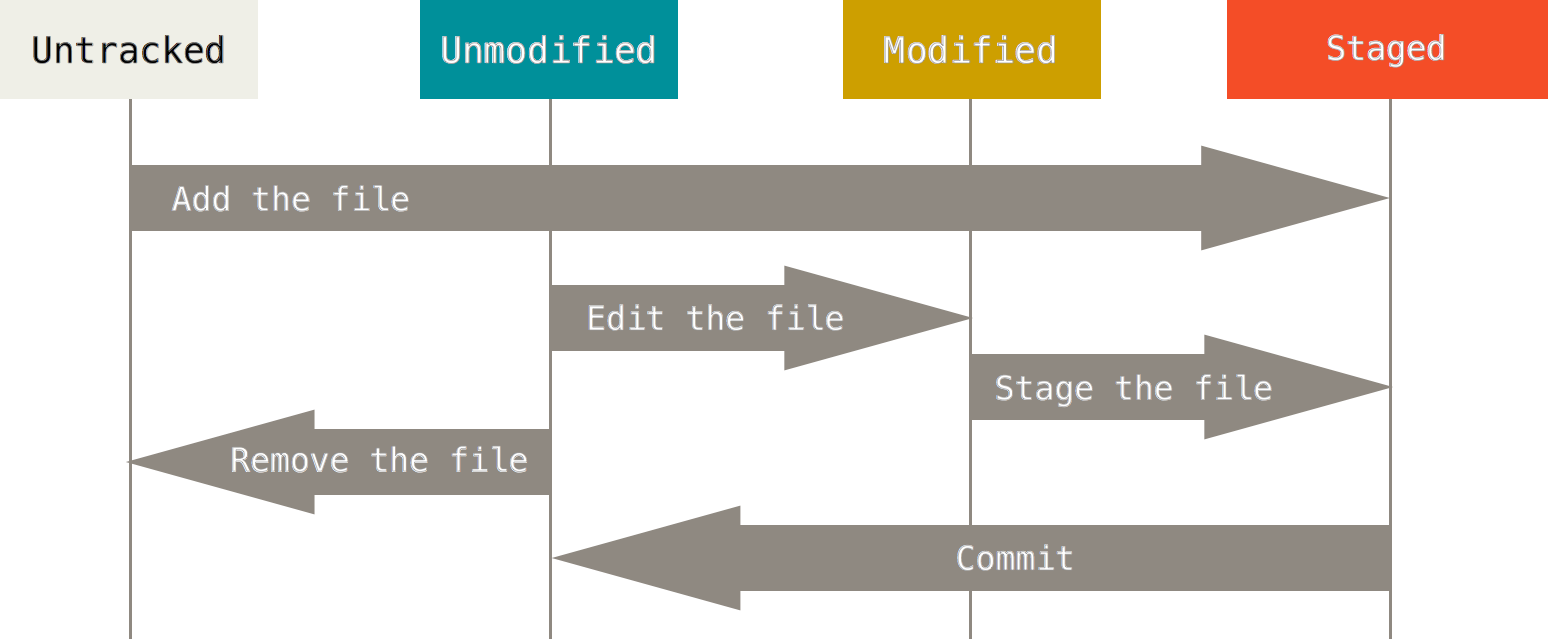
\includegraphics[height=6.5cm]{git_file-types}
		\captionsource{Możliwe stany pliku w systemie Git}{Oryginalna ilustracja angielska : \mbox{\url{https://git-scm.com/book/en/v2/Git-Basics-Recording-Changes-to-the-Repository}}}
		\label{fig:git_file-types}
	\end{figure}
	\FloatBarrier

	\paragraph{Etykiety}
	System Git umożliwia oznaczanie wybranych rewizji etykietami, zwanymi także znacznikami, za pomocą polecenia \textit{git tag}. Etykiety wykorzystywane są najczęściej do oznaczania ważnych wersji projektu, przede wszystkim na gałęzi produkcyjnej przy publikacji nowego wydania. Do wyszukania konkretnej rewizji w~historii projektu konieczne jest podanie skrótu SHA-1, identyfikującego daną rewizję, ale można w~tym celu posłużyć się znacznikiem. Dzięki temu odnalezienie istotnych wersji oprogramowania jest łatwiejsze.

	Etykiety nadawane rewizjom można podzielić na dwa typy:
	\begin{itemize}
		\item lekkie (ang. \textit{lightweight tags}) --- przechowujące jedynie skrót SHA-1 wskazywanej rewizji,
		\item opisane (ang. \textit{annotated tags}) --- zawierające poza skrótem SHA-1 rewizji także datę utworzenia, autora i~opcjonalnie dodatkowy komentarz.
	\end{itemize}

	\subsection{Gałęzie} \label{Galezie}
	W systemie Git istotną rolę pełnią gałęzie, będące w rzeczywistości wskaźnikami na rewizje.
	Każde repozytorium zawiera zaraz po utworzeniu dokładnie jedną, domyślną gałąź o nazwie \textit{master}. Wskazuje ona na najnowszą rewizję, czyli na samym początku na rewizję inicjującą. Po wykonaniu operacji zatwierdzenia wskaźnik aktualnej gałęzi automatycznie przesuwa się do przodu, na nowo powstałą rewizję. W~tym miejscu należy przypomnieć, że system Git przyporządkowuje rewizjom skróty \mbox{SHA-1}, służące jako identyfikatory. Dla każdej gałęzi przechowywany jest plik tekstowy, przechowujący skrót rewizji, na którą dana gałąź wskazuje. Oznacza to, że przesunięcie gałęzi sprowadza się jedynie do zmiany identyfikatora \mbox{SHA-1} w~pliku dotyczącym tej gałęzi.

	W systemie Git utworzenie nowej gałęzi jest niemalże natychmiastowe, ponieważ polega jedynie na dodaniu wskaźnika na rewizję. Wiąże się to ze stworzeniem pliku tekstowego, o takiej samej nazwie jak nazwa gałęzi, który zawierać będzie czterdziestoznakowy identyfikator wskazywanej rewizji. Operacja dodawania gałęzi jest bardzo szybka, nie wymaga bowiem kopiowania całego repozytorium.
	Wykonuje się ją poleceniem \textit{git branch}.

	Istnieje także szczególny wskaźnik HEAD, przechowujący informację o aktualnie aktywnej gałęzi. W odróżnieniu od zwykłej gałęzi nie wskazuje on na konkretną rewizję, lecz na gałąź. Jeżeli zostanie utworzona nowa rewizja, to wpis w pliku dotyczącym bieżącej gałęzi uaktualni się. W rezultacie HEAD będzie również wskazywał na najnowszą rewizję, choć zawartość jego pliku nie uległa zmianie~---~wskaźnik HEAD nadal wskazuje na aktywną gałąź.

	\begin{figure}[h]
		\centering
		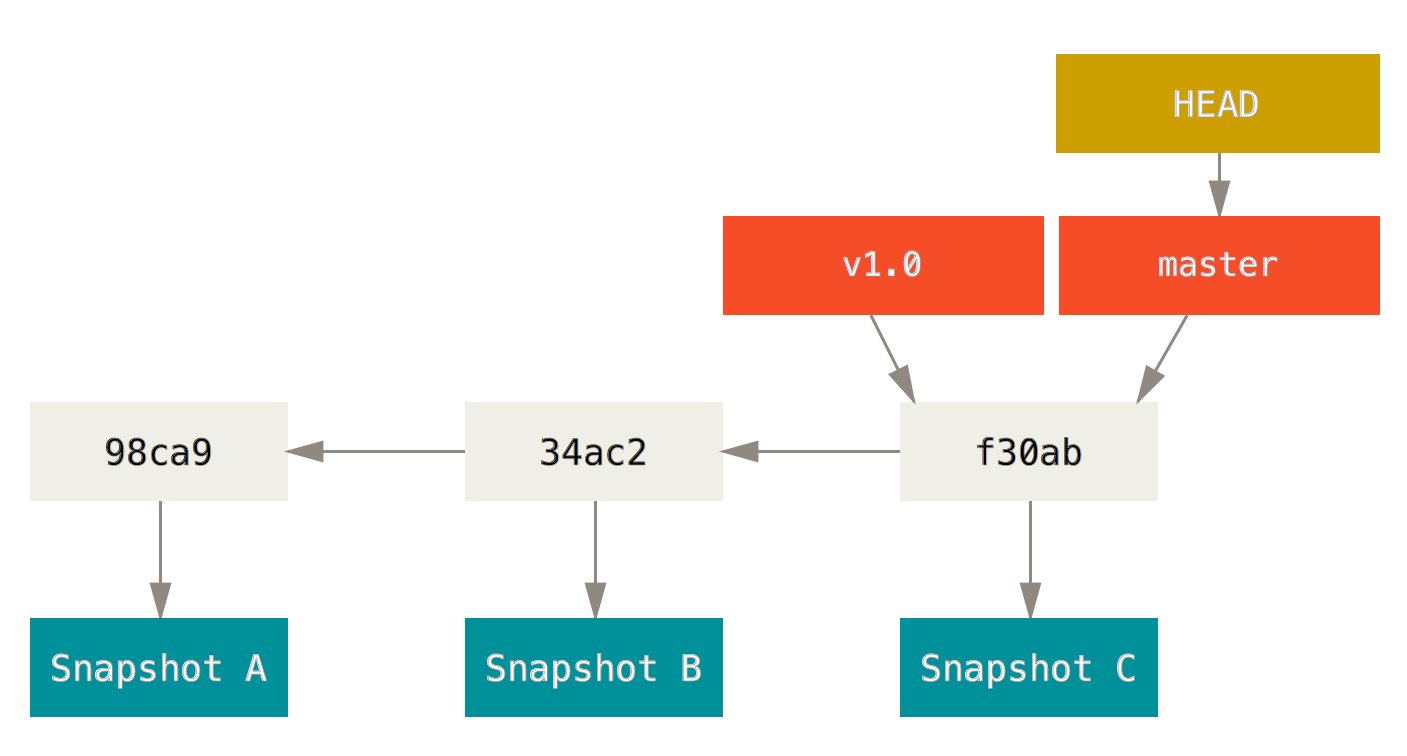
\includegraphics[width=12cm]{git_HEAD}
		\captionsource{Repozytorium zawierające trzy rewizje, z~bieżącą gałęzią \textit{master}}{\url{https://git-scm.com/book/en/v2/Git-Branching-Branches-in-a-Nutshell}}
		\label{fig:git_HEAD}
	\end{figure}

	Na rysunku \ref{fig:git_HEAD} przedstawione jest repozytorium, w którym utworzone zostały trzy rewizje. Ich skróty SHA-1 zaczynają się od następujących ciągów znaków: 98ca9, 34ac2 i f30ab. Każda z nich przechowuje zapamiętany stan projektu, czyli migawkę (ang. \textit{snapshot}). W~prezentowanym repozytorium są dwie gałęzie, \textit{v1.0} oraz \textit{master}. Wskaźnik symboliczny HEAD wskazuje na gałąź \textit{master}, co oznacza, że jest ona gałęzią aktywną.

	System Git umożliwia przełączanie się pomiędzy gałęziami za pomocą polecenia \textit{git checkout}. Przełączenie się na gałąź jest równoznaczne z~przywróceniem obszaru roboczego do stanu, jaki został zapisany we~wskazywanej przez nią rewizji. Możliwe jest również przełączenie się bezpośrednio na konkretną rewizję, nie wskazywaną przez żadną gałąź, poprzez podanie jej skrótu SHA-1. Spowoduje to przejście do stanu nazywanego w języku angielskim \textit{detached HEAD}, w~którym żadna gałąź nie jest gałęzią aktywną. Jeżeli w tym stanie wykonana zostanie operacja zatwierdzania, to utworzona rewizja nie będzie zawarta w~żadnej gałęzi, a~co za tym idzie może zostać łatwo utracona. W~związku z~tym nie należy pracować w stanie \textit{detached HEAD}. W~przypadku, w~którym konieczna jest kontynuacja projektu od konkretnej rewizji, należy najpierw utworzyć nową gałąź wskazującą na daną rewizję, a~następnie się na nią przełączyć.

	\subsubsection*{Łączenie gałęzi}
	Zmiany wprowadzone na osobnych gałęziach w systemie Git można połączyć, aby otrzymać wersję projektu zawierającą modyfikacje z kilku gałęzi. Istnieją dwa sposoby na wykonanie operacji łączenia, scalanie (ang. \textit{merge}) oraz zmiana bazy (ang.~\textit{rebase}). Ostateczny rezultat jest identyczny, różnica między tymi sposobami polega przede wszystkim na innej historii projektu.

	\paragraph{Scalanie}

	Łączenie gałęzi poprzez scalanie wykonywane jest poleceniem \textit{git merge}. Integrowanie zmian może być realizowane na gałęziach rozłącznych lub takich, z~których jedna jest zawarta w~drugiej. Przez zawieranie się gałęzi określa się sytuację, w~której jedna gałąź zawiera ciąg rewizji, a~druga składa się z identycznego ciągu do~którego dodane zostały nowe rewizje. Innymi słowy, z~pierwszej gałęzi można w~prostej linii dotrzeć do drugiej, podążając wzdłuż historii projektu.

	Wykonanie operacji scalania na gałęzi zawartej w dołączanej do niej gałęzi odbywa się poprzez przewinięcie do przodu (ang. \textit{fast forward}). Wskaźnik zawartej gałęzi jest przesuwany do najnowszej rewizji, wskazywanej przez gałąź dołączaną. Ilustracja~\ref{fig:git-merge_ff} przedstawia scalenie gałęzi \textit{master} z zawierającą ją gałęzią \textit{iss53}, które przewinęło wskaźnik gałęzi \textit{master} do przodu, nie tworząc przy tym nowej rewizji.

	\begin{figure}[h]
		\centering
		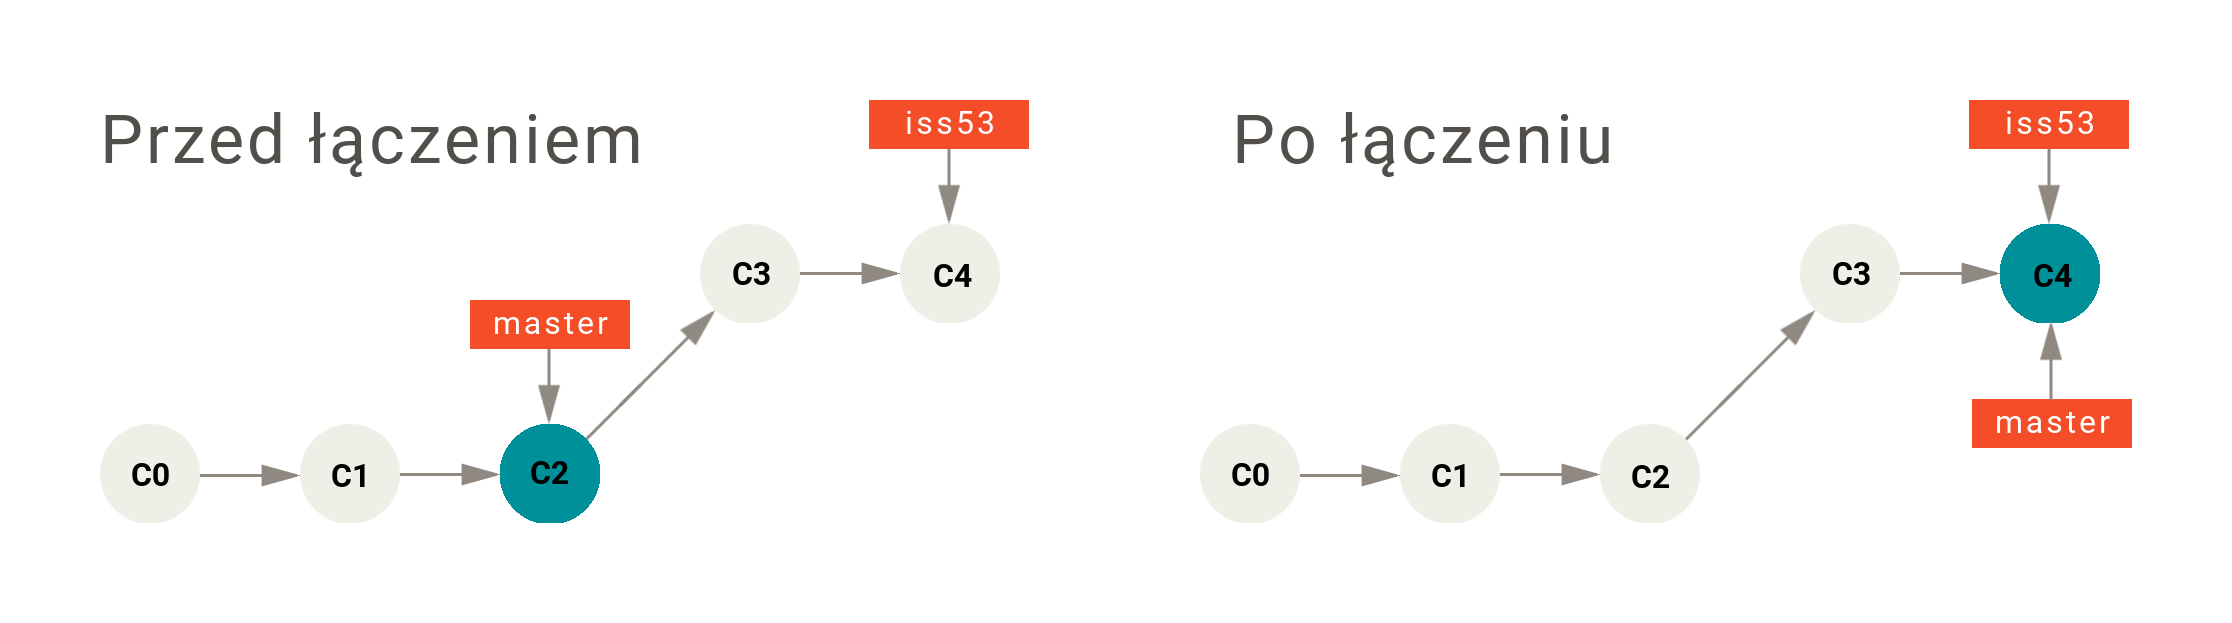
\includegraphics[width=14cm]{git-merge_ff}
		\caption{Działanie operacji scalania poprzez przewinięcie do przodu}
		\label{fig:git-merge_ff}
	\end{figure}

	W przypadku łączenia gałęzi rozłącznych, czyli takich, że~żadna nie jest zawarta w~drugiej, nie jest możliwe scalenie poprzez przewinięcie do~przodu. System Git ustala wówczas wspólnego przodka, czyli rewizję, od~której historie gałęzi się różnią, oraz rewizje wskazywane przez wskaźniki łączonych gałęzi. Na podstawie tych trzech migawek wykonywane jest scalenie trójstronne (ang.~\textit{three-way merge}), w~wyniku którego powstaje nowa rewizja. Jest ona szczególna, ponieważ posiada więcej niż jednego przodka.

	\begin{figure}[h]
		\centering
		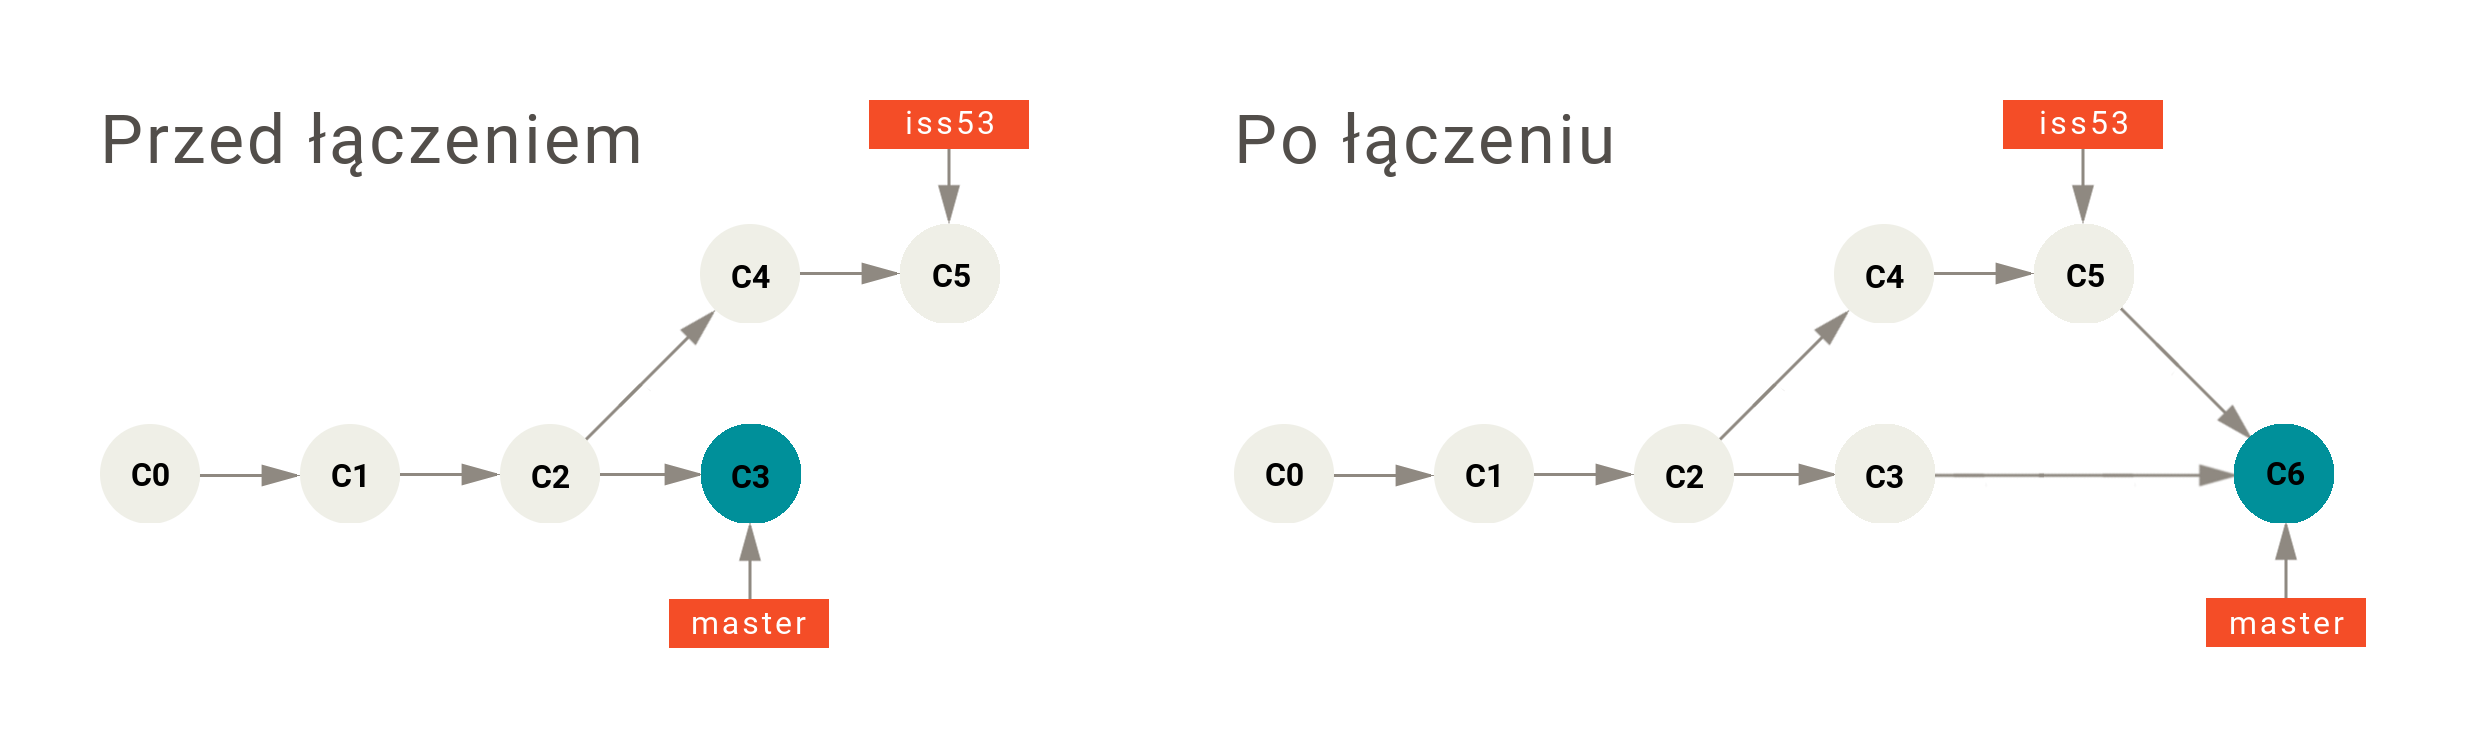
\includegraphics[width=15cm]{git-merge_no_ff}
		\caption{Działanie operacji scalania rozłącznych gałęzi}
		\label{fig:git-merge_no_ff}
	\end{figure}

	Przykład przeprowadzenia operacji scalania rozłącznych gałęzi jest przedstawiony na rysunku~\ref{fig:git-merge_no_ff}. Do gałęzi \textit{master}, która wcześniej wskazywała na rewizję C4, dołączone zostały zmiany z gałęzi \textit{iss53}. W wyniku tego powstała nowa rewizja C5.

	\FloatBarrier

	\paragraph{Zmiana bazy}

	Innym sposobem integracji zmian z różnych gałęzi jest zmiana bazy, wykonywana poleceniem \textit{git rebase}. System Git wyszukuje wspólnego przodka gałęzi i~sprawdza, jakie zmiany zostały przeprowadzone na gałęzi, którą chcemy dołączyć. Następnie zmiany te są nakładane na gałąź bazową. W rezultacie utworzone zostają nowe rewizje, a~gałąź bazowa jest zawarta w gałęzi, której baza została zmieniona. Można je teraz scalić poprzez przewinięcie do~przodu. Ostatecznie stan plików projektu jest identyczny z~tym, jaki powstałby w~wyniku operacji scalenia rozłącznych gałęzi. Jedyna różnica jest widoczna w~historii projektu~---~po zmianie bazy jest ona liniowa, a~w wyniku scalenia zawierałaby rozgałęzienia. Przykład działania operacji zmiany bazy przedstawiony jest na rysunku~\ref{fig:git-rebase}.

	\begin{figure}[h]
		\centering
		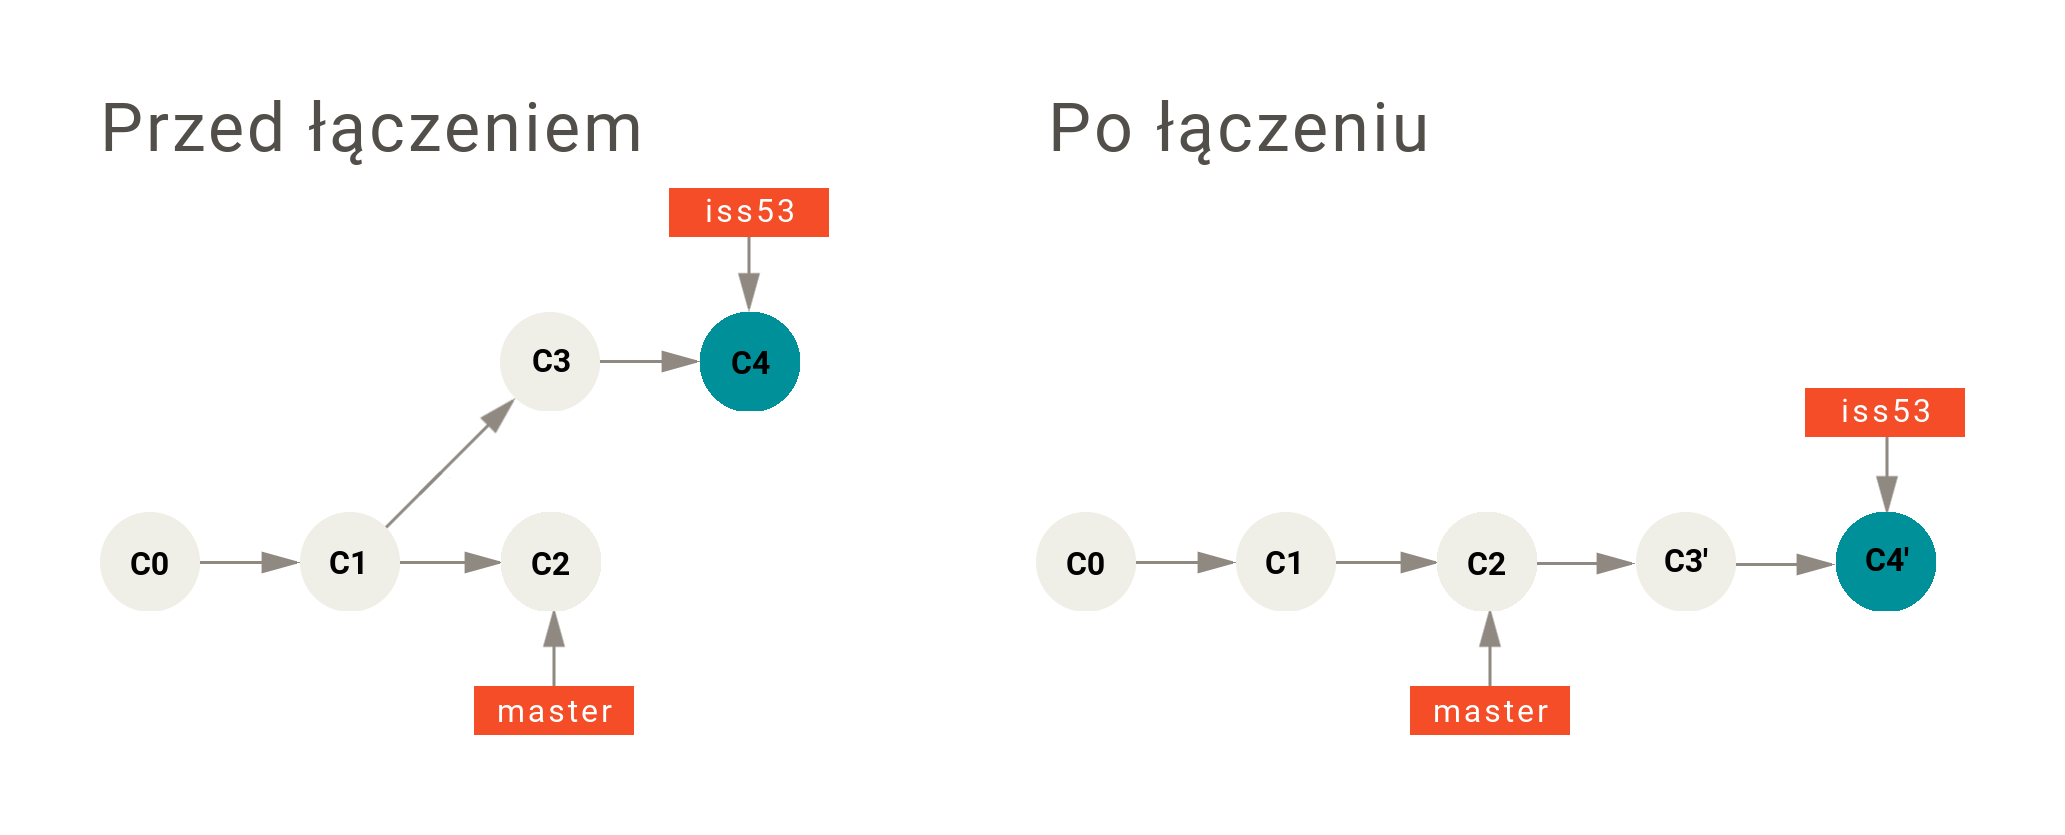
\includegraphics[width=13cm]{git-rebase}
		\caption{Działanie operacji zmiany bazy gałęzi \textit{iss53} }
		\label{fig:git-rebase}
	\end{figure}
	\FloatBarrier

	\subsection{Wycofywanie zmian}
	Jeżeli zajdzie potrzeba wycofania zaindeksowanych zmian lub usunięcia utworzonych rewizji, należy użyć komendy \textit{git reset} systemu Git, wywoływanej w~jednym z~trzech trybów:
	\begin{itemize}
		\item \textbf{\textit{soft}}~---~ aktywna gałąź (wskazywana przez HEAD) przesuwana jest do podanej jako parametr rewizji, a indeks i obszar roboczy pozostają bez zmian,
		\item \textbf{\textit{mixed}}~---~tryb domyślny, w którym aktywna gałąź przesuwana jest do podanej rewizji i dodatkowo zmieniany jest indeks (przywracany do stanu takiego jak w danej rewizji), a obszar roboczy pozostaje bez zmian,
		\item \textbf{\textit{hard}}~---~przesuwana jest aktywna gałąź, a zarówno indeks jak i~obszar roboczy są przywracane do stanu zapamiętanego w podanej rewizji (ten tryb może spowodować nieodwracalną utratę zmian, nawet tych zatwierdzonych).
	\end{itemize}
	Reasumując, polecenie \textit{git reset} z~opcją \textit{hard} wykonuje trzy kroki~---~cofa wskaźnik aktywnej gałęzi, zmienia indeks, a~następnie przywraca stan obszaru roboczego do~stanu zapisanego we wskazanej rewizji. W trybie \textit{mixed} pomijany jest ostatni krok, modyfikujący pliki w~katalogu roboczym. Z~kolei tryb \textit{soft} wykonuje tylko krok pierwszy.

	Komendę \textit{git reset} w trybie \textit{mixed} można wykorzystać do~wykluczenia zaindeksowanego pliku z~indeksu, a~z~opcją \textit{hard} do~usunięcia najnowszych rewizji. Za~pomocą tego polecenia wycofuje się także operację scalania, która utworzyła nową rewizję (nie dotyczy to scalania poprzez przewinięcie do~przodu).

	\subsection{Repozytoria zdalne}
	Do tej pory omówione pojęcia dotyczyły lokalnego repozytorium. System Git umożliwia pracę zespołową, do której niezbędne są zdalne repozytoria, udostępnione w~sieci. Służą one do~synchronizacji zmian w~projekcie, najczęściej wykonanych przez różne osoby. Korzystanie z~repozytorium zdalnego polega przede wszystkim na~pobieraniu i~przesyłaniu do~niego danych, dotyczących wersji projektu i~stanu plików.

	Jeżeli repozytorium lokalne powstało w wyniku wywołania komendy \textit{git clone}, to~jest kopią repozytorium zdalnego, podanego jako parametr polecenia i istnieje między nimi powiązanie.
	Z~jednym repozytorium lokalnym może być związanych kilka różnych repozytoriów zdalnych, które są najczęściej repozytoriami surowymi, czyli nie posiadającymi obszaru roboczego. Powiązanie dodaje się komendą {\textit{git~remote~add}, w~której określa się adres repozytorium zdalnego i~nadaje się mu dowolną nazwę. Domyślnie repozytorium zdalne, które zostało sklonowane, nosi nazwę \mbox{\textit{origin}}.

	\paragraph{Pobieranie zmian}
	Synchronizacja repozytorium lokalnego z repozytorium zdalnym wymaga pobrania danych z serwera. Służy do tego polecenie \textit{git pull}, które pobiera rewizje znajdujące się w repozytorium zdalnym, niewystępujące w~lokalnej historii projektu. Wywołanie tej komendy nie modyfikuje aktualnych plików w~obszarze roboczym, ponieważ zmiany z serwera zostają pobrane, ale nie zintegrowane z~bieżącą wersją.

	Repozytoria zdalne, tak jak zwykłe repozytoria lokalne, posiadają gałęzie (co~najmniej jedną, domyślnie nazwaną \textit{master}). Pobieranie zmian polega na pobraniu rewizji z konkretnej, zdalnej gałęzi. W celu dołączenia ich do własnej wersji projektu należy połączyć gałęzie~---~zdalną oraz lokalną. Operacja integrowania zmian przebiega w identyczny sposób, jak w~przypadku łączenia dwóch gałęzi lokalnych i~może być przeprowadzona poprzez scalanie lub zmianę bazy.

	Do pobrania zmian z repozytorium zdalnego można zamiast polecenia \textit{git fetch} użyć komendy \textit{git pull}, która najpierw pobiera brakujące rewizje, a następnie dołącza je do aktywnej gałęzi. Domyślnie operacja łączenia wykonywana jest poprzez scalanie, ale za pomocą odpowiedniego przełącznika można poinformować system Git, aby zamiast tego przeprowadził zmianę bazy.

	\paragraph{Wypychanie zmian}
	Przesyłanie rewizji utworzonych w lokalnym repozytorium na serwer realizowane jest poleceniem \textit{git push}, przyjmującym jako parametry nazwę zdalnego repozytorium oraz zdalną gałąź. Komenda zadziała tylko jeżeli na serwerze nie ma żadnych nowych, nie pobranych wcześniej zmian. W~przypadku, w~którym w~repozytorium zdalnym znajdują się rewizje nie dołączone do repozytorium lokalnego, próba wypchnięcia własnych zmian zostanie odrzucona. Konieczne będzie pobranie brakujących rewizji i~dołączenie ich do posiadanej wersji projektu. Przesłanie zmian do~repozytorium zdalnego jest możliwe dopiero gdy gałąź zdalna zawiera się w~lokalnej gałęzi.

	\paragraph{Gałęzie śledzące}
	Podczas wykonywania poleceń służących do pobierania lub wypychania rewizji konieczne jest określenie repozytorium zdalnego i~jego gałęzi, z~którą należy zsynchronizować zmiany. System Git umożliwia skonfigurowanie gałęzi lokalnej jako gałęzi śledzącej, mającej bezpośrednie powiązanie ze wskazaną gałęzią z repozytorium zdalnego. Dzięki temu, podczas wykonywania polecenia \textit{git pull} lub \textit{git push} z~gałęzi śledzącej, nie trzeba podawać żadnych parametrów, ponieważ synchronizacja domyślnie przeprowadzana jest z~gałęzią śledzoną.

	Lokalną gałąź śledzącą nazywa się w języku angielskim \textit{tracking branch}, a powiązaną z nią gałąź \textit{upstream branch}. W systemie Git istnieje też termin \textit{remote-tracking branch}, odnoszący się do referencji do zdalnej gałęzi. Wskazuje ona na~rewizję, na~jaką wskazywała dana zdalna gałąź podczas ostatniej komunikacji z~serwerem. W~przeciwieństwie do~zwykłych gałęzi tych referencji nie można samodzielnie przesunąć. Uaktualniają się automatycznie, na skutek wymiany danych z~repozytorium zdalnym.

	\section{Gitflow}

	Praca z~wykorzystaniem systemu Git może przebiegać w~zgodzie ze ściśle określonym cyklem. Ustalenie reguł, których będą przestrzegać wszyscy programiści pracujący nad danym projektem, może znacząco ułatwić synchronizację pracy i~pomóc w~sprawnym zarządzaniu i~wydawaniu nowych wersji oprogramowania. Jedną z~bardziej popularnych metodyk jest Gitflow, opracowana przez Vincenta Driessena. Określa ona cykl pracy, oparty na korzystaniu z~różnych gałęzi, z~których każda ma dokładnie zdefiniowaną rolę.

	\begin{figure}
		\centering
		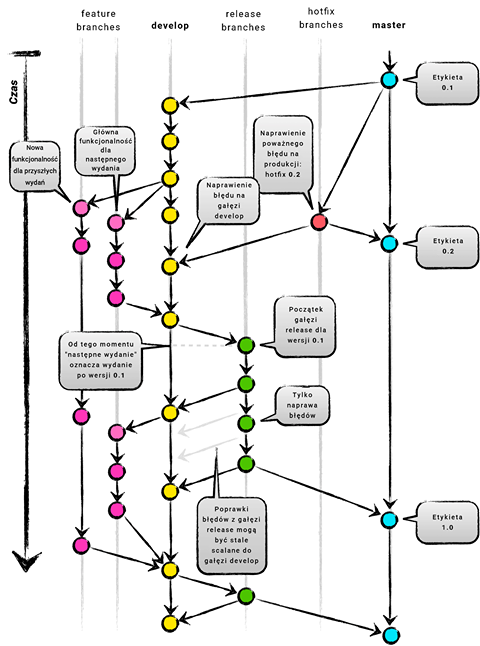
\includegraphics{gitflow}
		\captionsource{Typowy cykl pracy według Gitflow}{Oryginalna ilustracja angielska : \url{http://nvie.com/img/git-model@2x.pngS}}
		\label{fig:gitflow}
	\end{figure}

	\subsection{Podstawowe założenia}

	Zamiast korzystać jedynie z domyślnej gałęzi \textit{master}, Gitflow wykorzystuje dwie główne gałęzie do rejestrowania historii projektu. Jedną z nich jest gałąź produkcyjna \textit{master}, na której przechowywane są tylko oficjalne wydania (ang. \textit{release}). Druga służy jako gałąź deweloperska i jest nazywana \textit{develop}. Przeznaczona jest do integracji bieżących prac programistycznych i nowych funkcji.

	Obie wspomniane gałęzie w idealnym przypadku powinny składać się jedynie z~rewizji powstałych poprzez scalenie gałęzi (ang. \textit{merge commits}). Nie powinno się pracować i~zatwierdzać zmian bezpośrednio na~nich. Wszystkie modyfikacje kodu należy przeprowadzać na osobnych, dedykowanych gałęziach, tworzonych tymczasowo, w~dokładnie określonym celu. Koncepcja Gitflow wyróżnia trzy rodzaje takich gałęzi:
	\begin{itemize}
		\item wprowadzające nowe funkcje (ang. \textit{feature branch}),
		\item przygotowujące do opublikowania nowego wydania (ang. \textit{release branch}),
		\item zawierające niezbędne i szybkie poprawki (ang. \textit{hotfix branch}).
	\end{itemize}
	Z racji braku polskich odpowiedników nazw wymienionych powyżej gałęzi, w przypadku odniesienia do nich, w dalszej części pracy wykorzystywane będzie oryginalne nazewnictwo angielskie.

	Z technicznego punktu widzenia typy gałęzi wykorzystywanych w Gitflow niczym się nie różnią, są to zwykłe gałęzie systemu Git. Są one szczególne jedynie pod względem konkretnych celów, w~jakich są używane i~pewnych ograniczeń dotyczących procesu tworzenia i~łączenia ich. Każdy rodzaj może powstać jedynie przez rozgałęzienie z~określonej gałęzi (produkcyjnej lub deweloperskiej), a~na~koniec musi zostać połączony ze~ściśle ustaloną gałęzią lub gałęziami.

	\subsection{Rozszerzanie funkcjonalności}

	Jednym z podstawowych założeń Gitflow jest implementowanie każdej nowej funkcji oprogramowania na osobnej, dedykowanej gałęzi typu \textit{feature branch}, której nazwa powinna zaczynać się od ,,feature/''. Taka gałąź może powstać jedynie poprzez rozgałęzienie z~głównej gałęzi \textit{develop}. Z założenia ma składać się wyłącznie z rewizji zawierających zmiany dotyczące danej nowej funkcji i~istnieć tak długo, jak długo trwać będzie proces implementacji.

	Kiedy cel zostanie zrealizowany, gałąź typu \textit{feature branch} powinna być połączona z gałęzią \textit{develop}. Istotne jest aby operacja scalania nie została wykonana poprzez przewinięcie do przodu (ang. \textit{fast forward}), czyli zwykłe przesunięcie wskaźnika HEAD. Chodzi o to, by główna gałąź deweloperska nie zawierała wszystkich rewizji pochodzących z gałęzi dołączanej, lecz tylko jedną, powstałą jako łącznik dwóch gałęzi (ang. \textit{merge commit}). W przeciwnym wypadku określenie, które rewizje dotyczą wprowadzenia konkretnej funkcji, wymagałoby dokładnego przejrzenia zawieranych przez nie zmian. A w rezultacie znacznie trudniej byłoby usunąć pojedynczą funkcję z głównej gałęzi.

	Po włączeniu zmian z gałęzi przeznaczonej do implementacji nowej funkcji do głównej gałęzi \textit{develop}, należy usunąć tymczasową gałąź.

	\subsection{Przygotowywanie nowego wydania}

	Kiedy stan kodu aplikacji jest stabilny i działa zgodnie z oczekiwaniami, a wszystkie funkcje które powinny się znaleźć w nowym wydaniu oprogramowania są już zaimplementowane i włączone do głównej gałęzi deweloperskiej, należy rozpocząć proces publikacji nowej wersji. Zgodnie z koncepcją Gitflow, wszystkie niezbędne ostatnie poprawki i drobne zmiany dotyczące przygotowania nowego wydania, powinny zostać przeprowadzone na osobnej, specjalnie utworzonej w tym celu gałęzi, nazywanej \textit{release branch}.

	Tworzenie takiej gałęzi odbywa się poprzez rozgałęzienie z gałęzi \textit{develop}. W~tym momencie ustala się też numer wydania, czyli numer wersji publikowanego oprogramowania. Nazwa gałęzi powinna być formatu ,,release/numer-wydania''.
	Od tego momentu wszystkie zmiany zachodzące na~głównej gałęzi \textit{develop} będą dotyczyć następnej publikacji i~nie zostaną uwzględnione w aktualnym wydaniu. Dzięki utworzeniu gałęzi typu \textit{release} prace mogą iść dwutorowo,  poprzez przygotowywanie publikacji nowej wersji, oraz równolegle rozwijanie i~rozszerzanie funkcjonalności oprogramowania. Przygotowanie do wydania obejmuje korektę drobnych mankamentów, jak literówki i~inne niewielkie niedociągnięcia, a~także naprawę odkrytych podczas testowania błędów.

	W momencie, w którym oprogramowanie będzie już przygotowane do opublikowania, należy scalić gąłąź \textit{release} z~główną gałęzią produkcyjną \textit{master}. Analogicznie jak w~przypadku scalania gałęzi typu \textit{feature branch}, należy  zwrócić uwagę, aby operacja połączenia nie polegała na przewinięciu do przodu. Konieczne jest aby~w~wyniku jej wykonania utworzona została nowa rewizja. Należy jej nadać etykietę (ang. \textit{tag}) z~numerem wydania, aby ułatwić wyszukiwanie konkretnych wersji oprogramowania na gałęzi produkcyjnej. Następnie należy również scalić gałąź dotyczącą najnowszego, opublikowanego właśnie wydania, z~gałęzią \textit{develop}. Gałęzie typu \textit{relese} są tymczasowe, więc po włączeniu jej do obu głównych gałęzi należy ją usunąć.

	\subsection{Naprawa błędów wymagających szybkiego rozwiązania}

	Kolejnym typem gałęzi wykorzystywanych w~koncepcji Gitflow są gałęzie nazywane \textit{hotfix branches}, przeznaczone do~naprawy niecierpiących zwłoki błędów, odkrytych w~opublikowanym oprogramowaniu, najczęściej zgłoszonych przez użytkowników końcowych. Dotyczy to takich wad i~problemów, które są zbyt poważne, aby mogły zostać naprawione dopiero w~następnym wydaniu. W~przypadku mniej istotnych niedociągnięć wystarczy poprawić dane aspekty w~normalnym trybie pracy i~włączyć je do gałęzi \textit{develop}. Zostaną uwzględnione przy kolejnej publikacji przez gałąź typu \textit{release}.

	Gałąź typu \textit{hotfix} jest jedynym rodzajem gałęzi, który powstaje poprzez rozgałęzienie z~głównej gałęzi produkcyjnej \textit{master}. Jej nazwa powinna zaczynać się od~wyrażenia ,,hotfix/''. Taka gałąź zawiera tylko zmiany dotyczące naprawy wykrytego błędu, które powinny być wykonane w~możliwie najkrótszym czasie. Kiedy problem zostanie rozwiązany, przeznaczoną mu gałąź należy połączyć z~powrotem z~gałęzią \textit{master}. W~tym przypadku również należy dokonać łączenia nie poprzez przewijanie do przodu. W rezultacie na głównej gałęzi produkcyjnej powstaje nowa rewizja, której należy nadać etykietę z~kolejnym numerem wersji. Skutkiem jest publikacja nowego wydania oprogramowania, która, w~przeciwieństwie do~procesu z~wykorzystaniem gałęzi typu \textit{release}, nie była planowana.

	Kolejnym krokiem jest scalenie gałezi \textit{hotfix} z~główną gałęzią \textit{develop}. Jeżeli istnieje w~danym momencie gałąź typu \textit{release}, to do niej również należy włączyć zmiany dotyczące naprawy błędu. Na koniec należy usunąć tymczasową gałąź.

	\begin{figure}
		\centering
		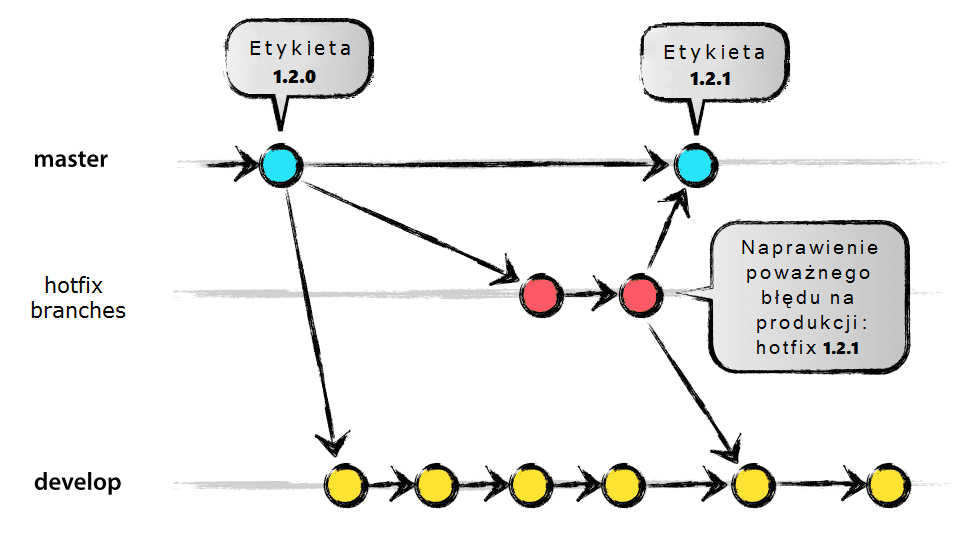
\includegraphics[height=5cm]{gitflow_hotfix}
		\captionsource{Wykorzystanie gałęzi typu \textit{hotfix}}{Oryginalna ilustracja angielska : \url{http://nvie.com/img/hotfix-branches@2x.png}}
		\label{fig:gitflow_hotfix}
	\end{figure}

	\chapter{Projekt}

	\section{Założenia}
		
	Głównym celem samouczka GITar-Hero jest zapoznanie użytkownika z~podstawowymi poleceniami systemu kontroli wersji Git, w~sposób przyjemny i~zrozumiały. Gra, przez połączenie nauki i~rozrywki, ma za zadanie zachęcić i~ułatwić proces uczenia się. Kolorowa i~ruchoma grafika 3D uatrakcyjnia tę naukę, a~możliwość zdobywania punktów i~naturalna chęć osiągnięcia jak najlepszego wyniku dodatkowo mobilizuje użytkownika.

	Z~założenia, ważniejsze od dogłębnego zrozumienia strony teoretycznej systemu Git, było nauczenie właściwego korzystania z~poleceń. Gra ma służyć jako samouczek, uczący praktycznego wykorzystania systemu wersji i~pokazujący typowy scenariusz, jaki najczęściej występuje podczas wytwarzania oprogramowania. Po~zagraniu w~grę użytkownik powinien już swobodnie wykonywać komendy systemu Git, zarówno pracując indywidualnie, jak i~podczas współpracy z~zespołem. 
	
	Celem było pokazanie, że~wbrew panującej powszechnie opinii, korzystanie z systemu kontroli wersji Git nie musi przysparzać problemów ani trudności. Ponadto gra ma przyzwyczaić użytkownika do korzystania z~wiersza poleceń. Opanowanie komend, jakie należy wprowadzać w~konsoli, z~reguły daje możliwość używania dowolnego programu z~graficznym interfejsem do obsługi systemu Git. W~drugą stronę taka zależność nie występuje. W~związku z~tym, tylko umiejętność korzystania z~systemu Git w~wierszu poleceń pozwala swobodnie korzystać z~tego systemu kontroli wersji, niezależnie od środowiska i~zainstalowanych programów.
	 
	\section{Przebieg gry}
	
	Gra zaczyna się od krótkiego wprowadzenia, informującego użytkownika, na czym będzie polegała rozgrywka i~do czego służą poszczególne elementy interfejsu. Po zapoznaniu się z~krótką instrukcją rozpoczyna się gra. U~góry, po prawej stronie, wyświetla się aktualne zadanie i~pierwszy krok, który należy wykonać. Z~założenia użytkownik nie zna poleceń systemu Git, dlatego automatycznie otwiera się zakładka pomocy, informująca czym jest repozytorium sytemu kontroli wersji i~jak je zainicjować. Pomoc zawiera wszystko, co gracz musi wiedzieć, aby poprawnie wykonać dany krok. Po wprowadzeniu przez niego właściwego polecenia i~zatwierdzeniu go poprzez przycisk Enter, aktualny krok zostaje zaliczony i~następuje przejście do kolejnego. Dodatkowo w katalogu projektu, po lewej stronie, pojawiają się aktualne pliki, jakie znajdują się w~folderze z~repozytorium. Poza tym akcje wykonywane na repozytorium są odwzorowywane przez grafikę 3D, która reaguje odpowiednio na wpisane komendy. Obrazuje to, jak wywołane polecenie wpływa na~stan repozytorium i~pozwala użytkownikowi lepiej zrozumieć skutki wykonywanych komend.

	Po wykonaniu przez użytkownika wszystkich kroków zadania, otrzymuje on punkty. Ich liczba jest zależna od czasu, jaki pozostał do końca zadania. Im szybciej gracz ukończy, tym więcej punktów dostanie. Możliwe jest także nie otrzymanie żadnej nagrody za wykonanie zadania, jeżeli przekroczony zostanie przydzielony do niego czas. Dodatkowo każda błędnie wprowadzona komenda skutkuje zmniejszeniem liczby posiadanych przez użytkownika punktów.
	
	Kolejne zadania, jakie musi wykonywać gracz, są zależne od jego umiejętności. Przechowywane są statystyki dotyczące wprowadzonych komend i~liczby popełnionych błędów. Jeżeli w krokach dotyczących określonego polecenia użytkownik często się mylił, to promowane będą zadania zawierające tę komendę. Nowe zagadnienia będą wdrażane dopiero, gdy wskaźnik znajomości polecenia będzie odpowiednio wysoki. Jest on wyliczany na podstawie liczby prób i~błędów, przy czym ostatnie próby mają większą wagę.
	
	Poziom trudności zadań stopniowo rośnie, zawierają one coraz więcej kroków. Jeżeli użytkownik nie będzie potrafił wykonać aktualnego kroku, może w~dowolnej chwili wpisać w~konsoli 'help'. Otworzy się wówczas pomoc i~gracz będzie mógł odnaleźć potrzebne mu informacji.

	Po przejściu całego scenariusza wyświetli się podsumowanie, zawierające liczbę zdobytych przez gracza punktów oraz podstawowe statystyki, takie jak informacja o~popełnionych błędach i~komendach, z~którymi miał najwięcej problemów. Ukończenie rozgrywki w krótkim czasie skutkuje przyznaniem użytkowniki dodatkowej nagrody, w~postaci bonusowych punktów.
	
	\section{Zadania}
	
	Scenariusz rozgrywki składa się z~zadań zawierających niezbędne komendy do typowego wykorzystania systemu kontroli wersji Git. Pierwszym terminem, z~jakim zapoznaje się użytkownik, jest repozytorium. Przedstawiane są dwie podstawowe metody pozyskania go~---~poprzez sklonowanie istniejącego lub przez założenie nowego w~wybranym folderze z~projektem. W~kolejnym etapie wprowadzane są pojęcia takie jak przestrzeń robocza, indeks, indeksowanie plików, zatwierdzanie zmian i~rewizja. Gracz uczy się rozróżniać pliki aktualne, zmodyfikowane, nieśledzone lub niezaindeksowane. Przed wprowadzeniem kolejnych poleceń i~terminów zadania koncentrują się na tej tematyce, aby użytkownik zdążył je dobrze opanować. 
	
	Po wykonaniu kilku zadań dotyczących wspomnianych wyżej zagadnień, użytkownik uczy się o~gałęziach, poznaje sposoby tworzenia ich i~przełączania się między nimi. Wprowadzane są też pojęcia takie jak gałąź tematyczna, poświęcona konkretnej dodatkowej funkcji aplikacji (ang. \textit{feature branch}). Przy okazji nadal utrwalane są komendy przedstawione w pierwszych zadaniach, dotyczące indeksowania plików i~zatwierdzania zmian. 

	Kolejnym etapem jest nauka łączenia gałęzi. Rozróżnione są przy tym odmienne sposoby na wykonanie tej operacji, takie jak scalanie i zmiana bazy. Następnie pojawia się podstawowy sposób wycofywania zmian i~usuwania wykonanych wcześniej rewizji.

	Kiedy użytkownik opanuje już komendy i~sposób pracy w~lokalnym repozytorium, zapoznaje się z~pojęciem zdalnego repozytorium oraz sposobami komunikacji i~synchronizacji z~nim. W~zadaniach pojawiają się komendy dotyczące ściągania i~przesyłania zmian. Poruszany jest także temat zdalnych gałęzi i~sposoby skonfigurowania lokalnej gałęzi śledzącej zdalną.
	
	Podczas nauki poleceń systemu Git użytkownik zapoznaje się też z~dobrymi praktykami i~metodyką Gitflow, co uczy go właściwych nawyków i~odpowiedniego porządkowania pracy nad projektem. Zaznajamia się z~koncepcją tworzenia osobnych gałęzi, przeznaczonych do implementacji nowych funkcji lub naprawy błędów.
	
	Zadania są podzielone na kroki, dzięki czemu gracz uczy się charakterystycznych sekwencji poleceń, które często występują w rzeczywistych sytuacjach. Ma to również na celu zautomatyzowanie zachowania użytkownika w~prawdziwych przypadkach, z~którymi może się spotkać w~domu lub pracy. W~systemie Git możliwe jest czasem użycie kilku różnych poleceń, aby osiągnąć ten sam rezultat. Zadania i~kroki dopuszczają wszystkie właściwe komendy.
	
	\subsection{Pomoc}
	
	Wszystkie materiały dydaktyczne znajdują się w~pomocy, podzielonej na zakładki, z~których każda dotyczy jednej komendy lub terminu. Jej treść wystarcza, aby osoba nie znająca poleceń systemu Git była w~stanie poprawnie wykonać zadania ze scenariusza rozgrywki. W~przypadku niektórych pojęć jest jednak bardziej obszerna i~wykracza poza wymaganą do przejścia gry wiedzę. Zawiera informacje, które uznano za szczególnie istotne i~przydatne do właściwego zrozumienia systemu Git.
	
	Za każdym razem, gdy podczas rozgrywki w jednym z kroków zadania pojawia się nowe polecenie, pomoc otwiera się automatycznie na odpowiedniej zakładce. Użytkownik może poświęcić dowolnie dużo czasu na zaznajomienie się z~jej treścią, a~ponadto w każdej chwili ma możliwość ponownego przeczytania informacji dotyczących wcześniejszych poleceń.  
	
	\subsection{Punkty za rozwiązanie}

	W projekcie wprowadzono elementy gamifikacji, takie jak punkty za rozwiązanie zadań. Mają one za zadanie zwiększyć zaangażowanie użytkownika. Z~każdym rozegraniem, gracz będzie starać się poprawić swój dotychczasowy wynik. W ten sposób co raz szybciej i~pewniej będzie korzystał z~poleceń systemu Git. Ponadto punkty wprowadzają element rywalizacji pomiędzy użytkownikami, którzy będą dążyć do osiągnięcia jak najlepszego wyniku.

	Punkty możliwe do otrzymania za zadanie obliczane są na podstawie liczby kroków~---~im bardziej złożone zadanie, tym wyżej punktowane. Ostateczna nagroda, jaka przyznawana jest graczowi za~wykonanie zadania, wyliczana jest jako procent maksymalnej liczby punktów, zależny od~czasu rozwiązywania. Dzięki temu użytkownik, który potrafi szybko wykonywać kolejne kroki, osiągnie lepszy wynik. Żeby zapobiec sytuacji, w~której prędkość stałaby się bardziej istotna niż dokładność, za~błędnie wprowadzone komendy gracz karany jest odjęciem określonej liczby punktów.
	
	\chapter{Implementacja}

	\section{Wykorzystane technologie}

	\subsection{Języki}

	\subsubsection{JavaScript}

	\subsubsection{GLSL}

	\subsection{Biblioteki}

	\subsubsection{Redux} \label{Redux}

	Wymagania dotyczące aplikacji przeglądarkowych stały się na tyle skomplikowane, że interfejs użytkownika jest bardzo złożony i może składać się z wielu elementów. Zarządzanie stanem takich aplikacji jest trudne, ponieważ występuje wiele zależności między komponentami. Może to doprowadzić do sytuacji, w której nie jest jasne co tak naprawdę się dzieje, a znalezienie błędów czy rozszerzenie funkcjonalności staje się zadaniem bardzo czasochłonnym.

	Jedną z bibliotek pomagających w rozwiązaniu tego problemu jest Redux. Jej głównym założeniem jest przejrzysty stan aplikacji, który może się zmieniać tylko w określonych momentach i~zawsze w~przewidywalny sposób.

	Stan w Reduxie zdefiniowany jest jako zwykły obiekt o~strukturze drzewa, zawierający wszystkie możliwe informacje, jakie są potrzebne aby jednoznacznie określić i móc odtworzyć identyczną sytuację w aplikacji. Nie może on być modyfikowany, jest tylko do odczytu. Jedynym sposobem na jego zmianę jest wyemitowanie akcji, będącej również obiektem zawierającym obowiązkowo pole typ i dowolne inne potrzebne atrybuty. Zadaniem akcji jest przejrzysty opis tego, co się wydarzyło w aplikacji, dzięki czemu dokładnie wiadomo czy i jak powinien zmienić się stan.

	Kluczowym elementem Reduxa są specyficzne funkcje, nazywane w języku angielskim \textit{reducers}, które definiują jak konkretna akcja wpływa na stan. Każda funkcja \textit{reducer} musi spełniać określone wymagania. Jako parametry przyjmuje zawsze tylko i~wyłącznie obecny stan aplikacji i wyemitowaną akcję, a zwraca nowy obiekt stanu, w jakim znajduje się aplikacja na skutek wykonanej akcji. Ważne jest także aby \textit{reducer} był przewidywalny i~deterministyczny. Oznacza to, że określony stan aplikacji i~określona akcja spowodują powstanie zawsze takiego samego stanu. Dodatkowo taka funkcja nie może mieć żadnych skutków ubocznych. W dużych projektach wskazane jest napisanie kilku takich funkcji, z~których każda wpływa tylko na określoną część stanu. Ułatwia to utrzymanie zrozumiałego kodu, który można łatwo rozwijać i~modyfikować.

	Podsumowując, Redux opiera się na trzech fundamentalnych zasadach:
	\begin{itemize}
		\item cały stan aplikacji jest opisany przez pojedynczy obiekt o strukturze drzewa,
		\item jedynym sposobem aby zmienić stan aplikacji jest wyemitowanie akcji,
		\item wpływ danej akcji na sposób przekształcenia stanu określają funkcje zwane \textit{reducers}.
	\end{itemize}

	Popularność biblioteki Redux zasłużenie rośnie, ze~względu na~prostotę i~korzyści, jakie daje przestrzeganie opisanych wyżej trzech podstawowych reguł. Zdecydowano się skorzystać z~tej biblioteki ponieważ jest łatwa w~użyciu i~pozwala w~wygodny sposób zarządzać stanem aplikacji.

	\subsubsection{React.js}

	 Jako bibliotekę do budowania interfejsu użytkownika wybrano bibliotekę React.
	 Została ona stworzona w 2013 roku przez zespół programistów Facebook'a, aby rozwiązać problem tworzenia dynamicznych aplikacji internetowcyh, w których nieustannie zmienia się to, co należy wyświetlać. Początkowo nie była ona ogólnodostępna, ale aktualnie jest rozpowszechniana na zasadzie otwartego oprogramowania (ang. \textit{open-source}).

   React opiera się na koncepcji niezależnych komponentów, nadających się do~wielokrotnego wykorzystania, z~których można komponować skomplikowane widoki. Są to obiekty JavaScript, reprezentujące fragmenty interfejsu użytkownika, mające określoną strukturę i~funkcjonalność. Każdy komponent musi implementować metodę \textit{render()}, odpowiedzialną za wyświetlenie komponentu w przeglądarce. W wartości zwracanej przez tę metodę mogą pojawić się zarówno znaczniki HTML jak i instancje zdefinowanych wcześniej komponentów. Aplikacje internetowe korzystające z biblioteki React budowane są zwykle na zasadzie drzewa komponentów. Tworzony jest jeden komponent nadrzędny, w którym zagnieżone są kolejne. Wzorzec ten pozwala zachować modułowość aplikacji.

   Komponenty czerpią wiedzę na temat wyświetlanych informacji z dwóch źródeł - właściwości (\textit{props}) oraz stanu (\textit{state}). Właściwości są obiektem reprezentującym parametry wejściowe podane podczas wywołania komponentu w komponencie nadrzędnym, natomiast stan jest obiektem widocznym i modyfikowalnym tylko wewnątrz danego komponentu. Zmiana stanu komponentu powoduje wywołanie jego metody \textit{render()} i, co za tym idzie, rekursywnego wywoływania metod \textit{render()} komponentów zagnieżdżonych. Efektem tej operacji jest modyfikacja odpowiednich węzłów obiektowego modelu dokumentu (ang. \textit{DOM}) przeglądarki i ostatecznie przerysowanie strony przez przeglądarkę. Należy zaznaczyć, że React jest dobrze zoptymalizowany pod kątem renderowania strony. Na szczególną uwagę zasługuje mechanizm wirtualnego obiektowego modelu dokumentu (ang. \textit{virtual DOM}). Polega on na utrzymywaniu kopii DOM reprezentowanej przez zwykłe obiekty JavaScript. Operacje na tych obiektach są znacznie mniej kosztowne, ponieważ nie zmuszają przeglądarki do ponownego renderowania strony. Właściwy DOM jest modyfikowany jedynie w przypadku stwierdzenia różnic między nim a wirtualnym DOM.

   Istotne ułatwienie dla procesu implementacji komponentów stanowi nakładka JSX. Jest to rozszerzenie składni języka JavaScript pozwalające w wygodny sposób używać tagów HTML oraz wywoływać wcześniej zdefiniowane komponenty w kodzie aplikacji. Używanie JSX jest zalecane przy tworzeniu aplikacji opartych o bibliotekę React przez samych jej twórców, ponieważ nie tylko ułatwia proces implementacji, ale również zwiększa czytelność kodu.

   Zdecydowano się na wykorzystanie biblioteki React.js, ponieważ dzięki abstrakcji operacji na elementach DOM na operacje na komponentach, pozwala ona przy stosunkowo niewielkim nakładzie pracy tworzyć aplikacje działające szybko i niezawodnie.

	\subsubsection{Babylon.js}

	Babylon.js jest otwartą biblioteką WebGL napisaną w TypeScript i~wykorzystywaną przede wszystkim do tworzenia gier wideo w~przeglądarkach. Pierwsza odsłona została wydana w~2013~roku. Głównymi twórcami są David Cotuhe oraz David Rousset. Jako, że Babylon.js jest silnikiem 3D, posiada wiele przydatnych narzędzi do tworzenia, wyświetlania i~teksturowania szkieletów w~przestrzeni. Przez to, że~kierowana jest głównie do twórców gier, posiada również dodatkowe funkcje takie jak generowanie krawędzi czy tworzenie obiektu na podstawie mapy wysokości. Ponadto zapewnia natywną detekcję kolizji, grawitację sceny oraz wbudowane kamery, takie jak kamera śledząca, automatycznie podążająca za obiektem.

	Jako alternatywa rozważana była biblioteka Three.js wydana w 2009 roku, również oparta na~webGL. Po zapoznaniu i~przetestowaniu obu silników wybór padł na Babylon.js. Przyczyniły się do tego przede wszystkim prostota użycia oraz płynność, którą zapewniał w przeciwieństwie do Three.js. Przy renderowaniu sceny o podobnej zawartości i szczegółowości, Babylon.js okazał się wydajniejszy. Poza tym biblioteka ta jest dobrze udokumentowana i~posiada bogatą bazę poradników, a~społeczność wykorzystująca tę bibliotekę jest bardzo liczna i~stale rośnie.

	\subsubsection{Pozostałe}

	\section{Scenariusz rozgrywki}

	\subsection{Struktura} \label{Struktura}

	Scenariusz rozgrywki to skierowany graf ważony, którego wierzchołki są~zadaniami, składającymi się~z~kilku kroków. Zdecydowano się na strukturę grafu ze~względu na~to, że~daje ona możliwość sekwencjonowania zadań, a~zarazem pozwala wprowadzić element losowości. Jeżeli z~wierzchołka dotyczącego jakiegoś zadania wychodzi kilka krawędzi, to kolejny węzeł, czyli kolejne zadanie, wybierane jest w~sposób losowy spośród sąsiadów aktualnego wierzchołka. Uwzględniane są przy~tym wagi krawędzi, generowane dynamicznie na podstawie statystyk gracza dotyczących znajomości poszczególnych zagadnień. Im~zadanie zawiera więcej kroków wymagających użycia problematycznych dla użytkownika poleceń, tym większą wagę ma~krawędź prowadząca do~tego węzła. A w rezultacie większe jest prawdopodobieństwo, że~wylosowane zostanie to zadanie.
	
	Dzięki takiej reprezentacji nigdy nie zdarzy się sytuacja, w~której następnym zadaniem będzie zadanie nieadekwatne do aktualnego stanu repozytorium, ale możliwe jest dynamiczne wybieranie zadań, uwzględniające umiejętności gracza.

	\subsubsection{Konstrukcja zadania}
	Pojedyncze zadanie reprezentowane jest w postaci obiektu, który składa się z pól opisanych poniżej.
	\begin{description}
	\item[Identyfikator] \hfill \\
		Unikalny numer zadania, na podstawie którego można dowiedzieć się, ile zadań zostało już wcześniej wykonanych.
		
	\item[Tytuł] \hfill \\
		Krótki tytuł zadania naprowadzający na poruszaną przez nie tematykę.
	
	\item[Opis] \hfill \\
		Opis zadania służy ukazaniu użytkownikowi celu oraz problemu, jaki należy rozwiązać w danym zadaniu. Może to być na przykład rozszerzenie funkcjonalności lub naprawa błędu.
		
	\item[Czas] \hfill \\
		Każde zadanie ma przydzielony czas, przeznaczony na jego wykonanie. Jeżeli gracz ukończy wszystkie kroki danego zadania w czasie krótszym niż ustalony, to otrzyma nagrodę w postaci punktów. Ich liczba zależna jest od liczby kroków zadania oraz wykorzystanego czasu.	
	
	\item[Lista kroków] \hfill \\
		Kluczowym elementem zadania jest uporządkowana lista kroków, które należy wykonać, aby rozwiązać zadanie i~przejść do kolejnego. Wykonanie kroku polega na wpisaniu odpowiedniej komendy systemu Git. Szczegółowy opis konstrukcji kroku w~kolejnej sekcji.
		
	\item[Zbiór identyfikatorów możliwych następników] \hfill \\
		Zbiór następników zawiera identyfikatory zadań, które mogą wystąpić po aktualnym. Hierarchia zadań ułożona jest w~postaci grafu skierowanego, tak więc~wszystkie wierzchołki, do~których istnieją krawędzie wychodzące z~wierzchołka reprezentującego dane zadanie, są~jego następnikami.	
	\end{description}

	\subsubsection{Konstrukcja kroku}
	
	\begin{description}
		\item[Typ] \hfill \\
		Określa, jakiej komendy systemu Git dany krok dotyczy. Obsługiwane typy to~m.in.~''COMMIT'' czy ''MERGE''. Na~podstawie typu poprawnie wykonanego kroku określana jest akcja, jaką należy wykonać po stronie grafiki 3D, by~odwzorować aktualny stan repozytorium.
		
		\item[Opis] \hfill \\
		Zawiera krótką informację, co należy zrobić, aby wykonać krok i~przejść do~kolejnego. 
		
		\item[Lista dozwolonych poleceń] \hfill \\
		Krok jest uznawany za~wykonany, gdy użytkownik wpisze w konsoli jedno z~poleceń z~listy dozwolonych komend i~zatwierdzi je. Lista musi zawierać co~najmniej jedno polecenie. Jeżeli jest ich więcej, to~są~to~komendy równoważne, mające identyczne działanie.
		
		\item[Etykiety] \hfill \\
		Do każdego kroku przypisana jest lista etykiet, określających jakich zagadnień on dotyczy. Krok posiada zawsze co~najmniej jedną etykietę, wskazującą komendę, której wymaga on do poprawnego wykonania. 
		
		Gdy użytkownik poprawnie zrealizuje dany krok, to zwiększany jest wskaźnik powodzenia dla wszystkich przypisanych do tego kroku etykiet. Poza wspomnianym wskaźnikiem przechowywana jest także ilość poprawnych wywołań komendy. Informacje te umożliwiają określenie stopnia, w jakim użytkownik opanował dane zagadnienie i~pozwalają ocenić, nad czym powinien jeszcze popracować. Statystyki te są brane pod uwagę przy losowaniu kolejnych zadań, ponieważ na ich podstawie wyliczana jest waga krawędzi.
		
		\item[Dodatkowe dane] \hfill \\
		Dodatkowe dane są charakterystyczne dla~każdego typu kroku i~mogą składać się z~różnych elementów. Dostarczają informację np.~o~nazwie wykonanej rewizji czy utworzonej gałęzi. Służą też do określenia jakie pliki powinny zostać dodane lub usunięte z~repozytorium. W~przypadku kroku dotyczącego polecenia \textit{git checkout} przechowują informację, czy~przełączenie powinno być zrealizowane na~konkretną gałąź czy~rewizję.
	\end{description}

	\subsubsection{Format danych}

	Jak opisano wcześniej, scenariusz rozgrywki to w istocie struktura drzewiasta, złożona z~zadań, przy~czym każde z~nich zawiera pewne informacje oraz uporządkowaną listę kroków. Tak złożony obiekt wymagał odpowiedniego i~wygodnego formatu do~przechowywania danych. Zdecydowano się~skorzystać z~formatu JSON, który doskonale nadaje się do tego celu. Pliki zapisane w~tym formacie można bezproblemowo odczytywać oraz modyfikować za~pomocą języka JavaScript.

	\subsection{Graficzne narzędzie do definiowania scenariuszy}

	\subsubsection{Motywacja}

	Aplikacja GITar Hero umożliwia przetwarzanie rozbudowanych scenariuszy, których ręczne tworzenie byłoby uciążliwe i  czasochłonne, a ponadto podatne na błędy. Dodawanie lub modyfikacja zadań wymagałaby znaczących nakładów pracy.
	Z tego względu zdecydowano się na korzystanie z narzędzia z graficznym interfejsem użytkownika, za pomocą którego można by było w prosty i wygodny sposób tworzyć grafy zadań oraz zapisywać je w formacie JSON.

	\subsubsection{Poszukiwanie gotowego rozwiązania}

	Początkowo zamierzano skorzystać z gotowego rozwiązania. Do tego zadania wytypowano aplikację \textit{directed-graph-creator} użytkownika cjrd [tu odnosnik do bibliografii i tam link] udostępnianą jako oprogramowanie o~otwartym źródle (ang. \textit{open source}) \footnote{Oprogramowanie udostępnione jest na licencji MIT/X, dzięki czemu istnieje nieograniczone prawo do używania, kopiowania, modyfikowania i~rozpowszechniania go. Jedynym wymogiem jest, by we wszystkich wersjach zachowano warunki licencyjne oraz informacje o autorze.}. Umożliwia ona tworzenie grafów skierowanych oraz~ich zapis do formatu JSON. Narzędzie to jest zaimplementowane w języku JavaScript i~korzysta z popularnej biblioteki~D3.js, która pozwala tworzyć dynamiczne i~interaktywne wizualizacje danych w~przeglądarkach internetowych.

	Jednakże aplikacja, w~formie w jakiej została udostępniona, nie wystarczała do zdefiniowania scenariusza rozgrywki. Każdy węzeł grafu mógł przechowywać tylko pojedynczy ciąg znaków. Potrzebne były zatem znaczne modyfikacje, umożliwiające zapisanie w pojedynczym węźle wszystkich niezbędnych informacji, które powinny się znaleźć w zadaniu. Zdecydowano się zatem stworzyć własne narzędzie do~tworzenia scenariusza zadań, bazujące na ogólnodostępnym \textit{direct-graph-creator}.

	\subsubsection{TaskCreator}

	Postanowiono przerobić wspomnianą wyżej aplikację. Została ona napisana tylko i wyłącznie w języku JavaScript, bez wykorzystania jakichkolwiek platform programistycznych (ang. \textit{frameworks}). Modyfikację utrudniał także fakt, że cały kod zawarty był w~jednym pliku. Postanowiono nie modyfikować struktury aplikacji i~dalszą część napisać również w czystym języku JavaScript. Dodano jedynie bibliotekę jQuery, która umożliwia łatwiejsze zarządzanie elementami drzewa DOM, czyli obiektowego modelu dokumentu. W~związku z~tym, że jest to aplikacja internetowa, potrzebny był serwer HTTP. W~tym celu użyto środowiska Node.js, wykorzystywanego do tworzenia wysoce skalowalnych aplikacji sieciowych.

	\begin{figure}
		\centering
		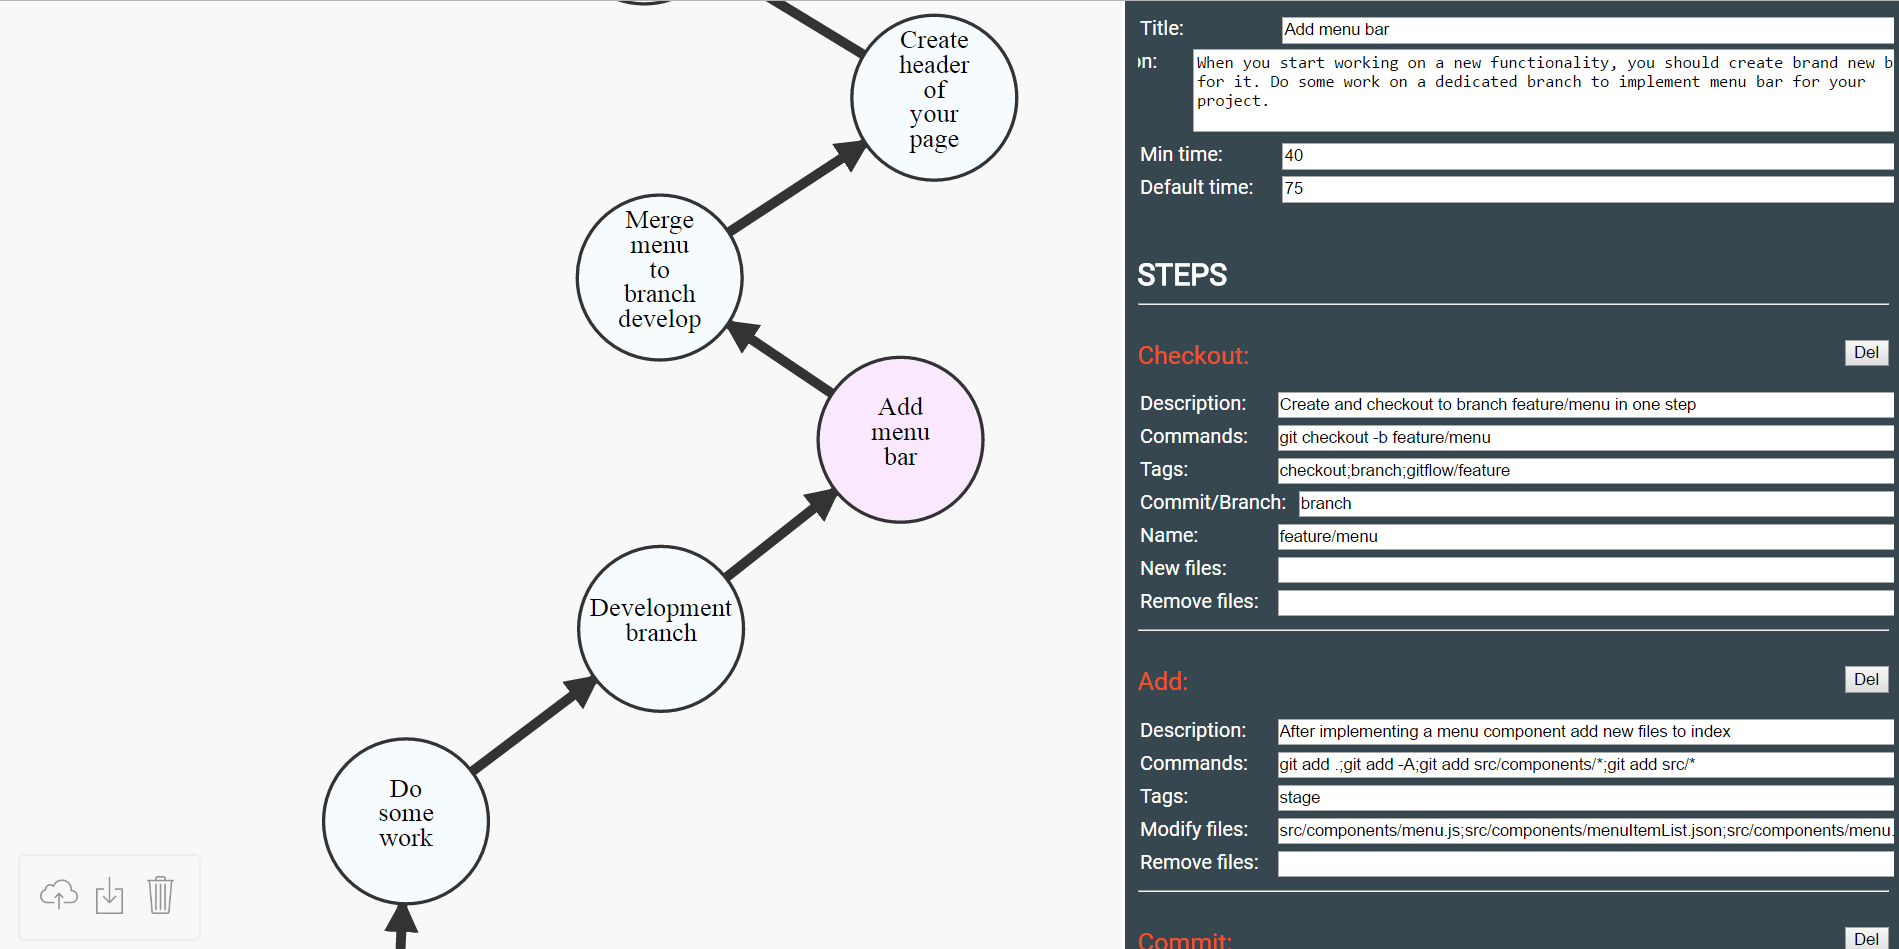
\includegraphics[width=12cm]{graphCreator01}
		\caption{Interfejs graficzny narzędzia TaskCreator}
		\label{fig:taskCreator}
	\end{figure}

	Największą modyfikacją było rozszerzenie interfejsu o dodatkowy panel boczny służący do wypełniania pól zadania i definiowania listy kroków. Jest on widoczny na rysunku~\ref{fig:taskCreator} po prawej stronie. Po~kliknięciu na węzeł grafu, reprezentujący pojedyncze zadanie, na bocznym panelu zostają wyświetlone wszystkie informacje dotyczącego wybranego elementu. Należą do nich między innymi tytuł, opis oraz czasy wykonania. Oczywiście wszystkie pola są edytowalne. W panelu istnieje również możliwość definiowania listy kroków, które trzeba zrealizować żeby wykonać zadanie. Aby dodać jeden z nich należy wybrać jego typ i kliknąć przycisk "Dodaj", a następnie wypełnić pola opisujące dany krok. Znajdują się tam atrybuty takie jak opis, lista komend spełniająca dany krok, etykiety opisujące wykonane czynności jak również dodatkowe parametry, charakterystyczne dla poszczególnych typów kroków.

	Aby dodać nowy węzeł grafu należy przytrzymać klawisz Shift i kliknąć myszką w wybrane miejsce. Żeby edytować wierzchołek należy go wybrać poprzez kliknięcie. Z kolei przytrzymanie klawisza Shift oraz wciśniętego lewego przycisku myszki a następnie przeciągniecie kursora znad jednego węzła na drugi utworzy skierowaną krawędź między nimi. Aby usunąć wybrany wierzchołek grafu bądź jego krawędź, należy go zaznaczyć kliknięciem oraz nacisnąć klawisz Delete.

	Stworzony w ten sposób graf zadań można zapisać do formatu JSON. W tym celu wystarczy kliknąć drugi przycisk w lewym dolnym rogu ekranu. Narzędzie wygeneruje strukturę grafu zrozumiałą dla aplikacji GITar Hero, określi zadanie inicjujące rozgrywkę i zapisze dane do pliku taskGraph.json. Zapisane w ten sposób grafy można wczytać ponownie do aplikacji TaskCreator naciskając pierwszy przycisk w lewym dolnym rogu ekranu i wybierając plik do wczytania.
	
	\section{Stan i jego tranzycje}
	
	\subsection{Wstęp}
	
	Stan naszej aplikacji został podzielony na pięć głównych części. Do każdej z~nich zdefiniowany został tzw. \textit{reducer} (więcej w sekcji \ref{Redux}) odpowiedzialny za tranzycje stanu w~zależności od typu akcji. Stan jest zatem obiektem posiadającym pięć kluczy, pod którymi zdefiniowane są obiekty definiujące stany określonych części aplikacji.
	
	Przy implementacji \textit{reducerów} zdecydowano się na popularny wzorzec wykorzystujący instrukcję \textit{switch}, sprawdzającą typ wyemitowanej akcji. Domyślnie zwracany jest niezmieniony fragment stanu, przekazany w pierwszym argumencie funkcji. Za pomocą słowa kluczowego \textit{case} zdefiniowane są natomiast wszystkie przypadki, w~których \textit{reducer} powinien zareagować wygenerowaniem nowego stanu.
	
	Zgodnie z wytycznymi twórców biblioteki \textit{Redux}, obiekt nowego stanu nie może być zmodyfikowanym obiektem poprzedniego stanu (stan powinien być stały i~nie podlegać mutacjom). Aby uzyskać taki efekt, posłużyliśmy się funkcją \textit{cloneDeep} z~pakietu \textit{lodash}, będącego zestawem pomocniczych funkcji służących do operacji na strukturach danych w JavaScript. Funkcja ta przyjmuje na wejściu obiekt, a~zwraca jego głęboką kopię. Jeżeli zatem stan wymaga tranzycji, to najpierw generowana jest jego głęboka kopia, a następnie jest modyfikowana i~zwracana jako nowy stan.
	
	\subsection{Zadania}
	
	Część stanu dotycząca zadań informuje przede wszystkim o aktualnym zadaniu wraz z~jego właściwościami. Dodatkowo zapamiętuje czas rozpoczęcia aktualnego zadania, co pozwala na obliczenie nagrody punktowej po wykonaniu go. Dostępna jest również informacja o powodzeniach i~niepowodzeniach w rozwiązywaniu zadań dotyczących określonych poleceń systemu Git.
	
	Poniżej opisane zostały akcje, które powodują wygenerowanie nowego stanu.
		
	\begin{description}
	\item[Nowa poprawna komenda z konsoli] \hfill \\
	Wyemitowanie akcji tego typu następuje na skutek poprawnego wykonania kroku zadania. W~rezultacie kolejny krok ustawiany jest w stanie jako aktywny oraz dodawana jest do statystyk informacja o poprawnie wykonanej komendzie danego rodzaju.
	\item[Nowa niepoprawna komenda z konsoli] \hfill \\
	Akcja tego typu zostanie wyemitowana, kiedy zostało zatwierdzone polecenie w konsoli, które nie należy do dozwolonych komend dla aktywnego kroku. W~efekcie w~stanie pojawi się informacja o~niepoprawnej próbie użycia polecenia danego typu.
	\item[Ostatni podpunkt zadania został wykonany] \hfill \\
	Wywoływana gdy dane zadanie zostało ukończone, czyli gdy ostatni krok został prawidłowo rozwiązany. \textit{Reducer} zareaguje wtedy wygenerowaniem nowego aktywnego zadania na podstawie przechowywanych statystyk dotyczących znajomości poleceń.
	\end{description}
		
	\subsection{Pomoc} \label{PomocStan}
	
	Osobną część stanu stanowią informacje dotyczące zakładki pomocy, dostępnej w~dolnej części strony. Pierwszą właściwość stanowi zmienna boolowska określająca, czy zakładka jest aktualnie otwarta, czy zamknięta (\textit{isOpen}). Druga właściwość to również zmienna boolowska, stanowiąca o~tym, czy pomoc ma otwierać się automatycznie, po pojawieniu się zadania zawierającego nowe polecenie (\textit{autoShowHelp}). Ostatnia wartość informuje o~aktywnej sekcji pomocy, widocznej o~ile zakładka jest otwarta (\textit{selectedTab}).
	
	Akcje, które powodują tranzycję stanu zakładki pomocy to:
	
	\begin{description}
	\item[Akcja nowej komendy z konsoli] \hfill \\
	Akcja tego typu wywołuje zmianę stanu, jeżeli treścią komendy jest słowo kluczowe "\textit{help}". \textit{Reducer} zmienia w efekcie wartość pola \textit{isOpen} na przeciwną w stosunku do aktualnej.
	
	\item[Akcja wyboru sekcji pomocy] \hfill \\
	Akcja tego typu informuje o wyborze aktywnej sekcji, a~w~niektórych przypadkach otwiera zakładkę pomocy. Jest ona emitowana podczas klikania w~tytuły sekcji w nawigacji zakładki pomocy, ale również gdy pojawi się krok dotyczący nowej komendy (aby wprowadzić gracza w~nowe zagadnienie). W~tym drugim przypadku w parametrach akcji przekazywana jest flaga \textit{auto}, ustawiona na~\textit{true}. Niezależnie od przyczyny wyemitowania akcji przekazywany jest identyfikator wybranej sekcji pomocy. \textit{Reducer} reaguje na akcję ustawiając wskazaną sekcję jako aktywną oraz otwierając zakładkę pomocy, o ile jest zamknięta i~spełniony jest następujący warunek~---~jeżeli automatyczne otwieranie pomocy jest wyłączone (flaga \textit{auto} jest ustawiona na \textit{false}), to źródłem akcji nie może być pojawienie się nowego polecenia.
	
	\item[Akcja zamknięcia zakładki pomocy] \hfill \\
	Wywoływana przez kliknięcie poza zakładką pomocy, wpisanie słowa kluczowego "\textit{help}" lub wciśnięcie przycisku \textit{ESC}, gdy zakładka jest otwarta. \textit{Reducer} otrzymując akcję tego typu ustawia pole \textit{isOpen} na wartość \textit{false}, co skutkuje zamknięciem pomocy.
	
	\item[Akcje nawigacji po sekcjach pomocy] \hfill \\
	Są to akcje przełączenia sekcji pomocy na poprzednią bądź następną. Naturalnie \textit{reducer} reaguje zmianem stanu pola dotyczącego aktywnej sekcji, ustawiając je na wartość poprzednią lub następną względem aktywnej.
	
	\item[Akcja zmiany opcji automatycznego włączania pomocy] \hfill \\
	Akcja ta emitowana jest kiedy gracz włącza lub wyłącza opcję automatycznego otwierania pomocy. \textit{Reducer} zmienia w efekcie wartość pola \textit{autoShowHelp} na~przeciwną w~stosunku do~aktualnej.
	\end{description}
	
	\subsection{Drzewo plików} \label{DrzewoStan}
	
	Aby symulować modyfikacje na plikach w repozytorium kontrolowanym przez gracza, potrzebna była reprezentacja tychże plików jako części stanu aplikacji. Struktura ta jest rekursywna i~umożliwia dowolne zagnieżdżanie plików w~katalogach. Każdy katalog jest reprezentowany przez obiekt, posiadający nazwę oraz zawartość w~formie tablicy obiektów. Pliki, również reprezentowane przez obiekty, zawierają obowiązkowo nazwę, ale także pola statusu oraz typu zmiany (nie posiadają pola zawartości). Część stanu reprezentująca katalog główny jest zatem tablicą obiektów o strukturze opisanej powyżej.
	
	Akcje, powodujące tranzycję stanu drzewa plików zostały opisane poniżej.
	
	\begin{description}
	\item[Akcja modyfikacji drzewa plików] \hfill \\
	Akcja ta została przygotowana, aby móc swobodnie operować na drzewie plików. We właściwościach akcji określane są pliki, które zostaną usunięte, zmodyfikowane lub dodane. \textit{Reducer} reaguje operacjami na strukturze reprezentującej drzewo plików dodając, usuwając i~modyfikując odpowiednie węzły.
	
	\item[Akcja zatwierdzenia poprawnej komendy w konsoli] \hfill \\
	Pliki w repozytorium zmieniają swoje statusy w~wyniku utworzenia nowej rewizji lub dodania plików do indeksu. W~związku z~faktem, że każdy \textit{reducer} informowany jest o~każdej wyemitowanej akcji, można w łatwy sposób stwierdzić żądanie utworzenia rewizji lub zaindeksowania plików z~poziomu \textit{reducera}. Wystarczy, że~po~otrzymaniu akcji zatwierdzenia w~konsoli poprawnej komendy sprawdzona zostanie składnia tego polecenia. Jeżeli odpowiada ona składni dodawania rewizji lub indeksowania zmian, \textit{reducer} wygeneruje nowy stan, odpowiadający drzewu plików z nowymi statusami. W przeciwnym wypadku zwrócony zostanie niezmieniony stan.
	\end{description}
	
	\subsection{Punkty}
	
	Część stanu dotycząca punktów zawiera informację o aktualnej liczbie punktów zdobytych przez gracza.
	
	\textit{Reducer} odpowiedzialny za stan punktów reaguje wygenerowaniem nowego stanu tylko w przypadku jednego typu akcji - akcji emitowanej, gdy ostatni krok zadania został poprawnie wykonany. W~takim przypadku liczony jest najpierw ułamek informujący o~tym, jaka część czasu przeznaczonego na zadanie została wykorzystana. Czas przydzielony do zadania jest liniowo zależny od liczby jego kroków. Następnie na podstawie tego stosunku i~maksymalnej liczby punktów, możliwych do uzyskania za to zadanie, wyliczana jest nagroda punktowa. Ostatnim krokiem jest dodanie otrzymanej nagrody do aktualnego wyniku i~zwrócenie nowego stanu.
	
	\subsection{Tutorial} \label{TutorialStan}
	
	Podczas pierwszego uruchomienia aplikacji gracz zostanie zapoznany z~zasadami gry przez wiadomości pojawiające się w~odpowiednich miejscach ekranu. Wyjaśniają one do czego służą poszczególne elementy interfejsu i~tłumaczą jak prawidłowo z~nich korzystać. Każda z takich wiadomości ma swój identyfikator. Stan przechowuje identyfikator aktualnie wyświetlanej wiadomości (lub wartość \textit{undefined}, gdy nie jest wyświetlana żadna wiadomość).
	
	Zostały przygotowane cztery wiadomości wprowadzające. \textit{Reducer} ma dostęp do tablicy \textit{tutorialsQueue}, w której zapisane są identyfikatory wiadomości zgodnie z~kolejnością ich wyświetlania. \textit{Reducer} generuje nowy stan w przypadku wyemitowania akcji informującej o~zamknięciu wiadomości. Zmienna \textit{current}, określająca aktualnie wyświetlaną wiadomość, zmienia się wtedy na wartość następną w~stosunku do~aktualnej w~tablicy \textit{tutorialsQueue}. W~efekcie akcja zamknięcia wiadomości w~przypadku pierwszych trzech powoduje przełączenie aktualnej wiadomości na~kolejną. Zamknięcie ostatniej wiadomości ustawia wartość zmiennej \textit{current} na~\textit{undefined}, co~oznacza, że~\textit{tutorial} został ukończony.

	\section{Komponenty graficzne}

	\subsection{Wstęp}

	Do połączenia komponentów interfejsu ze stanem aplikacji wykorzystano specjalny komponent \textit{Connect}, przygotowany przez twórców biblioteki \textit{Redux}. Pozwala on na~przekazanie konkretnych właściwości stanu do komponentu użytkownika. Żeby ustrukturyzować projekt, zdecydowano się na użycie popularnego wśród twórców aplikacji opartych o~\textit{React} i~\textit{Redux} wzorca, polegającego na podziale komponentów na~dwa typy: komponenty i~kontenery. Kontenery są niczym innym jak komponentami połączonymi ze stanem aplikacji poprzez \textit{Connect}.

	\subsection{Tutorial}

	W celu wyświetlenia tutoriala pojawiąjącego się po uruchomieniu aplikacji zaimplementowane zostały dwa komponenty~---~\textit{Tutorial} oraz \textit{TutorialItem}. Pierwszy z~nich z~założenia obejmuje całą treść strony, a~jako parametry wejściowe otrzymuje identyfikator aktualnie wyświetlanej wiadomości tutoriala oraz funkcję, która ma się wykonać po zamknięciu każdej wiadomości. Metoda renderująca tego komponentu obsługuje dwa stany, w zależności od wartości aktywnej wiadomości. 
	\begin{itemize}
		\item \textbf{Aktywna wiadomość jest ustawiona}~---~część zawartości komponentu zostanie przepuszczona przez filtr rozmywający (ang. \textit{blur}). Efekt ten osiągnięto przez dodanie klasy \textit{CSS} modyfikującej atrybut \textit{filter} na wszystkie elementy \textit{DOM} poza tymi, które chcemy wyróżnić (czyli elementem wiadomości oraz elementem, którego ta wiadomość dotyczy).
		\item \textbf{Aktywna wiadomość ma wartość \textit{undefined}}~---~żadna wiadomość nie jest wyświetlana, a~komponent renderuje swoją zawartość, nie wpływając w~żaden sposób na jej wygląd (elementy nie są rozmywane).
	\end{itemize}
	Komponent \textit{TutorialItem} służy temu, by nie dodawać klasy \textit{CSS} powodującej rozmycie na element którego dotyczy wiadomość. Przyjmuje on jeden parametr wejściowy, określający, czy jego zawartość powinna zostać wyłączona z procesu rozmywania.

	\subsection{Kontener aplikacji (App)}

	Kontener aplikacji (\textit{App}) stanowi korzeń drzewa komponentów interfejsu graficznego. Oznacza to, że jest on odpowiedzialny za~wyrenderowanie całego widoku aplikacji, wywołuje zatem wszystkie pozostałe komponenty. Cała zawartość kontenera zamknięta jest w~komponencie \textit{Provider}. Jest on dostarczony wraz z biblioteką \textit{Redux}, a~jego użycie jest wymagane dla poprawnego jej działania.

	Kontener ten korzysta z jednej właściwości stanu, mianowicie aktywnej wiadomości tutoriala. Właściwość ta jest przekazywana do komponentu \textit{Tutorial}, aby ten mógł wyświetlić odpowiednią wiadomość pomocniczą. Dodatkowo kontener aplikacji może emitować akcję wyłączenia wiadomości tutoriala (patrz: \ref{TutorialStan}). Metoda emitująca tę akcję jest przekazana do komponentu \textit{Tutorial}, aby umożliwić wyświetlanie kolejnych wiadomości. Jako zawartość komponentu \textit{Tutorial} przekazane są instancje wszystkich głównych komponentów gry, które zostały opisane w kolejnych podrodziałach.

	\subsection{Lista zadań}

	Lista zadań jest kontenerem korzystającym z dwóch właściwości stanu~---~zadań oraz tutoriala. Rolą tego kontenera jest wyświetlanie aktualnego zadania, wraz ze~wszystkimi jego krokami. W~tym celu zdefiniowano komponent pomocniczy \textit{Task}, umożliwiający wyświetlenie konkretnego zadania. Kontener listy zadań wyświetla zatem kolekcję zadań dostępną w~stanie, mapując każde z~nich na~wywołanie komponentu \textit{Task}. Dodatkowo wykorzystany został tutaj komponent pomocniczy, napisany przez twórców biblioteki \textit{React}, a~mianowicie \textit{ReactCSSTransitionGroup}. Dzięki umieszczeniu kolekcji elementów (w~tym przypadku komponentów \textit{Task}) w~komponencie \textit{ReactCSSTransitionGroup} możliwe jest zdefiniowanie animacji wejścia i~wyjścia elementu z~kolekcji przy pomocy arkuszy stylów \textit{CSS}.

	\subsection{Konsola}

	Konsola jest komponentem przyjmującym na wejściu cztery parametry. Pierwszy z~nich (\textit{enabled}) daje możliwość zablokowania konsoli, np.~w~przypadku, gdy tutorial nie został jeszcze ukończony. Kolejne dwa parametry (\textit{files}, \textit{branches}) to tablice wartości tekstowych, z~nazwami istniejących w~repozytorium plików oraz gałęzi. Nazwy te są potrzebne do działania funkcji autouzupełniania, znanej z~konsolowej wersji programu Git. Ostatni argument (\textit{onCommandEnter}) jest funkcją, która będzie wywołana, kiedy w~konsoli zostanie zatwierdzona komenda.

	Komponent konsoli wykorzystuje element \textit{input}, czyli pole tekstowe formularza \textit{HTML}. Niestety, element ten jest ograniczony pod kątem możliwości stylizowania za pomocą \textit{CSS}. W~związku z~tym zmiany w~tym polu śledzone są przy pomocy zdarzenia \textit{onChange}, a~sam element jest renderowany jako przezroczysty. Przy każdej zmianie wartości elementu \textit{input} jego wartość zostaje przepisana do innego, odpowiednio wystylizowanego elementu \textit{HTML}.

	Dodatkowo, aby upodobnić komponent do konsoli znanej z systemów operacyjnych, możliwe jest korzystanie z historii wpisywanych komend. Efekt ten osiągnięty został dzięki zapisywaniu każdego wprowadzanego polecenia w~stanie komponentu. Aby podnieść walory wizualne komponentu, historia jest czasowo wyświetlona nad obszarem wpisywania podczas używania klawiszy strzałek górnej i~dolnej.

	Dla ułatwienia szybkiej rozgrywki zaimplementowano mechanizm autouzupełniania dla nazw plików oraz gałęzi repozytorium. Wymagało to w~pierwszej kolejności zaprojektowania struktury drzewa podpowiedzi. Struktura ta opiera się na obiektach, z~których każdy posiada obowiązkowo właściwość \textit{pattern} oraz opcjonalnie właściwość \textit{children}. Pierwsza z~nich określa ciąg znaków, do których dopasowuje się dany węzeł drzewa oraz wszystkie jego następniki. Druga natomiast, o~ile jest zdefiniowana, przechowuje tablicę następników węzła.

	Zaimplementowano funkcje pomocnicze służące do generowania i~przeszukiwania drzewa autouzupełniania. Pierwsza z~nich umożliwia budowanie drzew autouzupełniania na podstawie wzoru zawierającego określone słowo kluczowe. Przykładowo, dla~wartości \textit{,,git checkout :branch:''} oraz tablicy wartości tekstowych, zawierającej nazwy istniejących gałęzi, wygenerowane zostanie drzewo autouzupełniania biorące pod uwagę polecenie tekstowe ,,\textit{git checkout}'' oraz listę gałęzi (z~uwzględnieniem możliwości nakładania się na siebie ich nazw). Mając do~dyspozycji listę dostępnych komend (w~odpowiedniej składni), listę istniejących gałęzi oraz plików, dzięki tej funkcji można zbudować drzewo, pozwalające w~dużym stopniu zasymulować autouzupełnianie znane z~konsoli systemowej. Funkcja przeszukująca dostaje na wejściu ciąg znaków (aktualną zawartość konsoli) i~rozpoczynając od korzenia przechodzi po węzłach, których wzór zawiera się tym ciągu znaków. Gdy nie ma już następnika spełniającego ten warunek, sprawdza, czy istnieje taki, którego wzór zawiera wejściowy ciąg znaków. Jeżeli istnieje i~jest to jedyny następnik spełniający ten warunek, to~jego wzór jest zwracany jako podpowiedź.

	Generowanie drzewa podpowiedzi jest stosunkowo kosztowną operacją, dlatego wykonywana jest ona tylko jeżeli zmieniła się lista plików lub gałęzi. Przeszukiwanie odbywa się za~każdym razem, gdy~podczas używania konsoli wciśnięty zostanie klawisz tabulacji.

	\subsection{Pomoc (HelpDrawer)}

	Zakładka pomocy jest kontenerem zawierającym komponent konsoli oraz treść materiałów dydaktycznych i~wskazówek przydatnych podczas rozwiązywania zadań. Kontener korzysta z~trzech właściwości stanu aplikacji:
	\begin{itemize}
		\item drzewa plików - potrzebnego do przekazania listy istniejących w~repozytorium plików do komponentu konsoli,
		\item aktywnej wiadomości tutoriala - wymaganej do uniemożliwienia interakcji z~konsolą do czasu zakończenia tutoriala,
		\item stanu zakładki pomocy - służącej do odpowiedniego wystylizowania zakładki w zależności od tego, czy jest otwarta, czy zamknięta.
	\end{itemize}
	  Gdy zakładka jest otwarta, wysuwa się z dolnej części ekranu. Efekt ten został osiągnięty przez animowanie właściwości \textit{translateY} elementu, które jest wysoce wydajne, ponieważ jest wykonywane na~karcie graficznej (w~odróżnieniu od właściwości takich jak \textit{top}, czy \textit{margin-top}, które pozwalałyby osiągnąć podobny efekt). 

	  Kontener pomocy emituje akcje związane ze zmianami stanu zakładki pomocy (patrz:~\ref{PomocStan}) oraz akcję zatwierdzenia nowej komendy (poprzez przekazanie komponentowi konsoli funkcji emitującej tę akcję).

	\subsection{Drzewo plików}

	Kontener drzewa plików jest odpowiedzialny za wyświetlenie informacji o~strukturze katalogu roboczego, w~którym znajduje się repozytorium. Korzysta on z~części stanu dotyczącej drzewa plików.

	Zaimplementowana została pomocnicza funkcja renderująca \textit{renderRecursively}, umożliwiająca wyświetlenie plików na~dowolnym poziomie zagnieżdżenia. W~jej pierwszym wywołaniu jako argument podawane jest drzewo plików ze~stanu. Ma~ono strukturę tablicy (patrz:~\ref{DrzewoStan}). Dla każdego z~elementów funkcja sprawdza czy jest on plikiem, czy katalogiem. Jeżeli jest to~plik, to~zwrócony zostaje pomocniczy komponent pliku (odpowiedzialny za dodanie odpowiedniej ikony oraz koloru, w~zależności od~statusu pliku). W~przypadku katalogu zwracany jest nowy element \textit{HTML} wyświetlający jego nazwę, a~zawartość folderu wyświetlana jest poprzez rekursywne wywołanie funkcji \textit{renderRecursively}.

	Poziom zagnieżdżenia plików został przedstawiony za pomocą łączących je linii oraz odpowiednich wcięć z~lewej strony.

	\subsection{Canvas}

	Komponent \textit{Canvas} stanowi połączenie między architekturą opartą o~komponenty \textit{React} i~stan aplikacji, a~moduł 3D, zaimplementowany z~wykorzystaniem biblioteki \textit{Babylon.js}.

	Pierwszym zadaniem komponentu jest wstawienie do obiektowego modelu dokumentu elementu \textit{canvas}, który umożliwia rysowanie przy pomocy technologii \textit{WebGL}. Założono dodatkowo, że~po~utworzeniu tego elementu, powinien on~być modyfikowalny tylko z~poziomu modułu 3D (metoda \textit{render} komponentu powinna wykonać się tylko raz). Efekt ten osiągnięto implementując metodę \textit{shouldComponentUpdate} i zwracając w niej zawsze wartość \textit{false}. \textit{React} pozwala na zaimplementowanie tej metody w przypadku, w~którym użytkownik chce zablokować przerysowanie komponentu po zmianie jego stanu lub parametrów wejściowych. Po utworzeniu elementu \textit{canvas}, inicjowany jest moduł 3D, do którego element ten przekazywany jest jako argument.

	Parametrem wejściowym komponentu \textit{Canvas} jest obiekt \textit{store}, zawierający stan aplikacji i~umożliwiający reagowanie na~emitowane akcje. Jest on~wykorzystywany do~przekazywania modułowi~3D informacji o~zmianach, które pojawiły się w~repozytorium.

	\section{Grafika 3D}

	\subsection{Repozytorium 3D}
	Aby odwzorowywać stan repozytorium na ekranie został stworzony odpowiedni kontroler. Ma on za zadanie reagować na realizowane przez użytkownika komendy i zarządzać elementami grafiki 3D. Nasłuchuje na wykonywane akcje i w zależności od ich typu dodaje, usuwa bądź modyfikuje elementy na scenie. Kontroler ten zawiera informacje na temat utworzonych gałęzi repozytorium oraz wskaźnik HEAD, o którym więcej w sekcji 4.4.5.

	\subsection{Branch}
	Obiekt 3D reprezentujący gałąź systemu git jest tworzony przy pomocy funkcji CreateTube z biblioteki Babylon.js. Funkcja ta generuje siatkę wierzchołków, na podstawie podanej listy punktów określających ścieżkę, w kształcie tuby. Pozwala również na określenie średnicy oraz szczegółowości siatki. Parametry te zostały dobrane w taki sposób, aby wygenerować tubę, której przekrój przypomina koło przy jednoczesnym zachowaniu jak najmniejszej liczby użytych wierzchołków. Jedna gałąź może składać się z dwóch rodzajów siatki. Pierwsza z nich reprezentuje główny człon. Ścieżka użyta do jej wygenerowania zawiera tylko dwa punkty wyznaczające początek i koniec tuby. Dzięki temu można osiągnąć dowolnie długi odcinek nie zwiększając przy tym liczby wierzchołków. Drugi rodzaj siatki wykorzystywany jest do wygenerowania tuby będącej łącznikiem między gałęziami. Łącznik branchy zostaje stworzony w momencie tworzenia nowej gałęzi lub łączenia dwóch gałęzi w akcji merge. Do wyznaczenia ścieżki skorzystano z funkcji pomocniczej generującą krzywą Beziera. Funkcja ta przyjmuje cztery punkty na podstawie których wyznaczy tablicę punktów tworzących linie. Jako pierwszy punkt podane jest miejsce początku nowej gałęzi, dwa kolejne punkty służą do określenia kształtu linii. Jako ostatni punkt podawany jest początkowy punkt głównego członu nowej gałęzi. Dodatkowym parametrem jest ilość wygenerowanych punktów określającym szczegółowość linii. Dzięki tej funkcji otrzymano tablicę punktów, która została użyta do określenia kształtu łącznika. Następnie sprawdzane jest, czy na wygenerowanej ścieżce nie znajduje się inna gałąź. Jeśli tak, to zwiększana jest jej wysokość, a następnie zmniejszana do początkowej wartości tak, aby przejść nad nią.

	Dla gałęzi zaimplementowano animacje wydłużania oraz skracania. Dla głównego członu polega ona na przesunięciu ostatniego punktu ścieżki, a następnie zaktualizowaniu bufora wierzchołków. Służy do tego ta samo funkcja, co do tworzenia początkowej siatki wierzchołków, lecz z dodatkowym parametrem, będącym instancją obiektu, którego bufor należy zmienić. W przypadku łącznika gałęzi animacja jest bardziej skomplikowana. Aby osiągnąć efekt rozwijania oraz w związku z tym, że nie można zmieniać rozmiaru bufora wierzchołków, należy wszystkie punkty ścieżki przesuwać na jej początek, a następnie rozwijać w kierunku końca ścieżki. Podobnie jak w pierwszej animacji przy każdym nowym stanie ścieżki należy zaktualizować bufor wierzchołków.

	Na gałąź nałożono standardowy materiał. Jest to klasa z biblioteki Babylon.js reprezentująca uniwersalny shader.  Można w nim określić takie właściwości jak kolor, przezroczystość oraz tekstury.

	Na końcu każdej gałęzi wyświetlany jest tekst z nazwą gałęzi o kolorze białym. Jego pozycję ustawiono na referencję do ostatniego punktu gałęzi dzięki czemu tekst zawsze podąża za wydłużającą lub skracającą się gałęzią.


	%standardowy material
	% tuba
	% connectory
	% tekst
	% husaku i imosiaku

	\subsection{Commit}
	Zatwierdzenie zmian w repozytorium git w grafice trójwymiarowej jest przedstawione w postaci kuli umieszczonej na gałęzi, której dotyczy. Funkcja CreateSphere pochodząca z babylon'a buduje siatkę wierzchołków w kształcie sfery o określonej średnicy oraz teselacji. Przy wartości teselacji równej szesnaście powierzchnia obiektu wygląda na wygładzoną. W momencie utworzenia kuli  pojawia się nad nią napis z wiadomością przekazywaną przy zatwierdzaniu zmian, którego kolor jest niewiele jaśniejszy niż kolor samego obiektu. Ponadto może również zostać dodany tekst z numerem wersji tzw. tag, znajdujący się nieco powyżej tekstu z wiadomością. Sam tekst jest wyświetlany tylko dla 'commitów' na gałęzi, na której aktualnie znajduje się użytkownik, a jego pojawienie się , czy ukrycie jest animowane.

	 W kwestii wyglądu wobec kuli zastosowane te same zabiegi co do gałęzi, na której jest umieszczona. Posiada ten sam kolor, materiał oraz obramowanie.

	Z obiektem ukazującym zatwierdzenie zmian związane są animacje takie, jak pojawienie się czy zniknięcie z wybuchem cząsteczek. Pierwsza z nich trwa 0.4 sekundy i polega na modyfikowaniu skali z wykorzystaniem funkcji generującej krzywą Beziera, tak by przypominało to sprężanie i rozprężanie, co tworzy ciekawy efekt wizualny. Obiekt potwierdzający zmiany może zostać usunięty, jeżeli użytkownik wykonana akcja zresetowania repozytorium do jakiejś wcześniejszej zmiany. W tym celu napisano efektowną animację z wybuchem cząsteczek stałych, będących niewielkimi kulami. Cząsteczki są w tym samym kolorze co 'commit'. W przypadku tworzenia stałych cząsteczek w formie wybuchu skorzystano z mechanizmów babylona, który ułatwia pracę z cząsteczkami. Na początku tworzona jest figura z 500 cząsteczek, będących sferami. Następnie definiowana jest funkcja wykonywana dla każdej cząsteczki, w której określa się prędkość oraz kierunek jej rozchodzenia. Cząsteczki rozchodzą się dynamicznie w kształcie kuli, a w każdej klatce zmniejszana jest ich skala, by zanikały w czasie, wszystko to daje efekt eksplozji ciała, co urozmaica doznania wizualne.

	\subsection{Tekst}
	Tekst w grafice 3D jest ukazany w postaci dwuwymiarowej z opcją billboard w trybie  wszystkich osi. Oznacza to, że niezależnie jak ustawiona będzie kamera tekst będzie się odpowiednio obracał w kierunku kamery.

	Aby utworzyć tekst w babylon należy zastosować kilka operacji, które w projekcie zebrano w jedną klasę. Na początku tworzona jest płaszczyzna o rozmiarach, wyliczonych na podstawie rozmiaru pojedynczego znaku, pomnożonego przez ilość liter w tekście. Do wygenerowania tekstury z tekstem użyto klasy DynamicTexture z biblioteki Babylon.js. Po utworzeniu instancji tej klasy wywoływana była jej funkcja rysująca tekst na teksturze. Umożliwia ona określenie miejsca, czcionki, koloru tekstu oraz przezroczystości tła. Kolor tekstu ustawiany jest w zależności od obiektu nad którym się znajduje, a tło jest w pełni przezroczyste. W kolejnym kroku powstaje materiał z biblioteki Babylon.js , w którym jako tekstura, określająca kolor oraz nieprzezroczystości, jest wcześniej utworzona tekstura.

	Dla tekstu zdefiniowano dwie animacje pojawienia się i zniknięcia. Przy ich tworzeniu zastosowano gotowe mechanizmy z biblioteki babylon. Aby uzyskać efekt pojawiania się modyfikowana jest wartość przezroczystości materiału płaszczyzny od zera do jeden w ciągu jednej sekundy, natomiast przy znikaniu, następuje mechanizm odwrotny, polegający na zmianie tej samej wartości od jeden do zera. W ten sposób uzyskano efekt 'gaśnięcia'.

	Obiekt ten jest wykorzystywany przy ukazywaniu wiadomości i tagów z wersją dotyczących zatwierdzenia zmian, a także przy wyświetlaniu nazw gałęzi.


 	% repo 3d jak kontroler akcji husaku i imosiaku
 	% branch i animacje, akcje husaku i imosiaku
 	% colors i shaders husaku ?
 	% ground husaku ?
 	% background i particles magda?

	\subsection{Kamera}

	Nieodzownym elementem w projekcie z grafiką 3D jest kamera. W przypadku GitHero kamera jest kamerą śledzącą obiekt i rozszerza standardowe możliwości 'FollowCamera' z babylon'a. Określa się dla niej rotację, odległość oraz wysokość z której ma spoglądać na śledzony obiekt, a także prędkość podążania, czy przyspieszenie. Kamera powinna podążać zawsze za aktywną gałęzią. W systemie git aktywna gałąź przetrzymywana jest we wskaźniku HEAD, dlatego postanowiono odwzorować jego działanie. Stworzono obiekt HEAD posiadający informację na jaki obiekt wskazuję. Najczęściej jest to gałąź repozytorium, ale może też wskazywać na komita. Aby ułatwić podążanie kamery za HEADem stworzono klasę abstrakcyjną FollowObject i rozszerzono o nią obiekt HEAD. Po wskazaniu obiektu za którym powinna podążać kamera na obiekt jaki wskazuje HEAD można było w łatwy sposób zmieniać aktywne gałęzie i dzięki implementacji gotowej kamery z biblioteki babylon.js kamera podążała samoistnie do wskazanego obiektu. Niestety gdy zmieniano aktywną gałąź znajdującą się daleko od aktualnej gałęzi kamera zmieniała gwałtownie swoją pozycję i nie poruszała się płynnie. Postanowiono dodać dodatkowy, obiekt do klasy FollowObject nazwany CameraTarget, na który to była skierowana kamera i podążała za nim. W każdej klatce sprawdzana jest pozycja CameraTarget i obiektu na który wskazuje HEAD. Gdy obie pozycje się różnią następuje płynne przesunięcie CameraTarget na pozycję obiektu wskazanego przez HEAD. W wypadku gdy wskazywanym obiektem jest gałąź pobierana zostaje pozycja najdalej wysuniętego punktu gałęzi wzdłuż osi Z. Dzięki temu kamera podąża za aktywnym obiektem w sposób płynny. Aby obiekt CameraTarget nie był widoczny po utworzeniu zostaje usunięty ze sceny dzięki czemu nie jest wywoływana funkcja rysująca go. Aby móc sprawdzić jak wygląda wizualizacja całego repozytorium zaimplementowano możliwość oddalenia kamery przy użyciu przewijania myszką. W momencie przewijania w tył kamera zwiększa swoją wysokość, prędkość oraz przyspieszenie aż do momentu osiągnięcia z góry ustalonej maksymalnej wysokości. Następnie zaczyna zmniejszać swoją pozycję wzdłuż osi Z aż do momentu dotarcia do początku repozytorium. W momencie przewijania w przód następuje odwrotny proces aż do dotarcia do końca aktywnej gałęzi. W czasie zmiany pozycji kamery wzdłuż osi Z następuję zmiana pozycji wzdłuż tej samej osi obiektu na który kamera spogląda o taką samą wartość dzięki czemu kamera skierowana jest ciągle pod takim samym kątem wzdłuż osi X. Dzięki temu, że kamera nie spogląda na konkretny obiekt repozytorium tylko na CameraTarget nie zmienia się pozycja obiektu na który wskazuje HEAD.

	\subsection{Lecący kod ?}

	Aby odwzorować ciągłe przybywanie nowego kodu w projekcie postanowiono stworzyć komponent imitujący lecący tekst. Do tego celu stworzono płaszczyznę z wykorzystaniem funkcji CreateGround z biblioteki Babylon.js. Jako parametry podaje się w niej rozmiar płaszczyzny oraz ilość wierzchołków użytych do jej wygenerowania. Następnie nałożono na nią materiał w którym to zaimplementowano własny shader wierzchołków oraz shader pikseli. Aby kod był zawsze widoczny i nie znikał gdy kamera porusza się do przodu w każdej klatce wartość Z wektora pozycji płaszczyzny ustawiana jest na wartość Z wektora pozycji kamery. Głównymi parametrami przekazywanymi do shadera wierzchołków jest pozycja i koordynaty tekstury. Dodatkowo dostarczane są macierze świata, widoku i projekcji. Aby sprawić wrażenie falowania kodu postanowiono nadać płaszczyźnie wypukłości. Z tego powodu przekazywana jest do shadera wierzchołków monochromatyczna tekstura zawierająca informację o wysokości wierzchołków zwaną mapą wysokości. Aby obliczyć końcową pozycję wierzchołka pobierana jest wartość kanału czerwonego z mapy wysokości z miejsca określonego koordynatami tekstury. Wartość ta przyjmuje wartości od 0 do 1. Jest to za mała wartość aby można było zauważyć różnicę w wysokości płaszczyzny dlatego jest ona przemnażana przez z góry ustaloną wartość określającą maksymalną wysokość. Następnie obliczona wysokość dodawana jest do wartości y wektora pozycji wierzchołka. Otrzymana pozycja jest pozycją wierzchołka w modelu płaszczyzny. Aby ustawić wierzchołki w świecie oraz uwzględnić ustawienie i właściwości kamery pozycja wierzchołka mnożona jest przez macierz świata, widoku i projekcji. Z shadera wierzchołków do shadera pikseli przekazywana jest pozycja wierzchołka w modelu płaszczyzny (nie przemnożona przez macierz świata, widoku i projekcji) oraz koordynaty tekstury. Dodatkowo przekazywana jest pozycja kamery oraz tekstura z kodem. Aby stworzyć wrażenie poruszającego się tekstu w shaderze wierzchołków do koordynatów tekstury dodawane jest przesunięcie obliczane w każdej klatce w klasie materiału. Na samym początku pobierany jest kolor z tekstury kodu z użyciem przesuniętych koordynatów tekstury. Następnie sprawdzane jest czy pobrany kolor jest kolorem czarnym (wartości R,G i B wynoszą zero). Gdy jest to prawdą piksel zostaje pominięty. Dzięki temu na ekranie wyświetlany jest tylko kod z tekstury (brak czarnego tła). Gdy kolor pobrany z tekstury nie jest czarny oznacza to że jest to piksel kodu i należy ko narysować. Aby sprawić wrażenie delikatnego pojawiania się kodu zaimplementowano efekt mgły. Kod znajdujący się daleko od kamery delikatnie zaczyna przybierać kolor tła. Na początku obliczana jest głębokość piksela na podstawie koordynatów piksela. Wartość 'Z' koordynatów piksela określająca głębokość piksela dzielona jest przez wartość W określającą projekcje. Dzięki temu wiemy jak daleko od kamery jest część kodu reprezentowana przez ten piksel. Dzięki temu, że płaszczyzna jest w stałem odległości od kamery, możemy określić wartość współczynnika mgły. Dla pikseli reprezentujących koniec kodu współczynnik ten wynosi 1. Czym mniejsza głębokość tym współczynnik zmniejsza się osiągając wartość zero w momencie gdy głębokość jest mniejsza od z góry ustalonej wartości. Dzięki temu można powoli ukrywać tylko końcówkę kodu. Ostateczna wartość koloru piksela obliczana jest na podstawie współczynnika mgły. Gdy jego wartość jest bliższa 1 wtedy piksel posiada kolor tła. Gdy wartość wynosi 0 wtedy jako kolor używany jest kolor tekstury. W wartościach pośrednich kolor jest liniowo interpolowany. Do tego celu skorzystano z wbudowanej funkcji w WebGl o nazwie 'mix'. Jako pierwszy parametr został podany kolor tekstury, drugim parametrem jest kolor tła, a jako trzeci parametr podany został współczynnik mgły. Aby móc w łatwy sposób wyłączyć efekty takie jak falowanie i przesuwanie kodu do shedera przekazywane są również dodatkowe parametry określające czy wykonać dany efekt.

	\subsection{Tło}

	\chapter{Podsumowanie}

	\appendix

	\chapter{Przewodnik użytkownika}

	Praktyczne info dla opornego użytkownika, jak ma korzystać, między innymi że jest opcja scrolla aby oddalić, jakie przyciski do obsługi helpa itp. itd., krótki opis fragmentu rozgrywki co się dzieje po czym i dlaczego i jak ma na to reagować użytkownik i takie tam.

	\backmatter

\end{document}
